% Monograph LaTeX Template for UFSC based on:
%
% 1. https://github.com/royertiago/tcc
% 2. http://portal.bu.ufsc.br/normalizacao/
% 3. https://github.com/AdrianoRuseler/abntex2-ufsc

% You need to run `pdfTeX` 5 times on the following order: 1. `pdfTeX`, 2. `biber`, 3. `pdfTeX` 4.
% `pdfTeX` 5. `pdfTeX` 6. `biber` 7. `pdfTeX`, when the bibliography includes a cyclic reference to
% another bibliography, so we need a last pass to fix the bibliography undefined references.

% Includes and fixes several `abntex2` class problems
% Must be included before loading class
%----------------------------------------------------------------------------------------
%   PACKAGES AND OTHER DOCUMENT CONFIGURATIONS BEFORE LOADING abntex2
%----------------------------------------------------------------------------------------

% Uncomment the line `\englishtrue` to set the document default language to english.
%
% Is it possible to keep my translation together with original text?
% https://tex.stackexchange.com/questions/5076/is-it-possible-to-keep-my-translation-together-with-original-text
\newif\ifenglish\englishfalse
% \englishtrue

% How to expand \ifthenelse so that it can be used in \parshape?
% https://tex.stackexchange.com/questions/131002/how-to-expand-ifthenelse-so-that-it-can-be-used-in-parshape
\newcommand{\lang}[2]{\ifenglish#1\else#2\fi}

% Disable the empty pages automatically put by memoir class, except the ones by \cleardoublepage
% \PassOptionsToClass{openany}{memoir}

% How to make \PassOptionsToPackage add the option as the last option?
% https://tex.stackexchange.com/questions/385895/how-to-make-passoptionstopackage-add-the-option-as-the-last
\ifenglish
    \newcommand{\swapcontents}[2]{#1 #2}

    \PassOptionsToPackage{language=english}{biblatex}
    \PassOptionsToPackage{brazil,main=english,spanish,french}{babel}
\else
    \newcommand{\swapcontents}[2]{#2 #1}

    \PassOptionsToPackage{language=brazil}{biblatex}
    \PassOptionsToPackage{main=brazil,english,spanish,french}{babel}
\fi




% Applying options to already loaded package
% https://tex.stackexchange.com/questions/124049/applying-options-to-already-loaded-package
%
% For web links and paths with \path{..} and \url{https://www.python.org/downloads/}
% https://tex.stackexchange.com/questions/3033/forcing-linebreaks-in-url
% ftp://tug.ctan.org/pub/tex-archive/macros/latex/contrib/hyperref/doc/options.pdf
\PassOptionsToPackage{hyphens}{url}

% Use its macro adjustwidth* to extend tables out of outer text border.
% https://tex.stackexchange.com/questions/366155/how-to-write-a-table-a-little-larger-than-the-paragraphs-with-centered-columns
\PassOptionsToPackage{strict}{changepage}

% Linked footnotes are not supported inside environment `tabularx', because they
% uses the optional argument of \footnotetext
% http://ctan.sharelatex.com/tex-archive/macros/latex/contrib/hyperref/README.pdf
\PassOptionsToPackage{hyperfootnotes=false}{hyperref}

% The class `abntex2` loads the `enumitem` package with options.
%
% With the package option shortlabels you can use an enumerate-like syntax, where A, a, I, i and 1
% stand for \Alph*, \alph*, \Roman*, \roman* and \arabic*. This is intended mainly as a sort of
% compatibility mode with the enumerate package, and therefore the following special rule applies:
% if the very first option (at any level) is not recognized as a valid key, then it will be
% considered a label with the enumerate-like syntax.
%
% No spacing between enumerated items with \usepackage{enumerate}
% https://tex.stackexchange.com/questions/119919/no-spacing-between-enumerated-items-with-usepackageenumerate
\PassOptionsToPackage{shortlabels}{enumitem}

% Fixes `pdfTeX warning (ext4): destination with the same identifier (name{figure.1.1}) has been
% already used, duplicate ignored`.
%
% The `abntex2` package loads the `hyperref` package, however there are several packages which are
% required to be loaded after and before `hyperref`.
%
% Which packages should be loaded after hyperref instead of before?
% https://tex.stackexchange.com/questions/1863/which-packages-should-be-loaded-after-hyperref-instead-of-before
%
% Hyperref is loaded by the class, and I need to load packages that are supposed to be loaded before
% https://tex.stackexchange.com/questions/50846/hyperref-is-loaded-by-the-class-and-i-need-to-load-packages-that-are-supposed-t
%
% Using \BeforePackage to load a package before hyperref does not work
% https://tex.stackexchange.com/questions/51094/using-beforepackage-to-load-a-package-before-hyperref-does-not-work
\RequirePackage{scrlfile}
\AfterClass{memoir}
{
    \RequirePackage{float}
}

% The class `abntex2` loads the package `enumitem`, but `paralist` must be loaded before it
% https://tex.stackexchange.com/questions/162799/compilation-error-when-including-enumitem-and-paralist-packages
\AfterClass{memoir}
{
    % How to make horizontal lists?
    % https://tex.stackexchange.com/questions/146306/how-to-make-horizontal-lists
    \RequirePackage{paralist}
}

% Biblatex error: Incompatible backref package
% https://tex.stackexchange.com/questions/383054/biblatex-error-incompatible-backref-package
%
% backreferencing in classicthesis package does not work
% https://tex.stackexchange.com/questions/115828/backreferencing-in-classicthesis-package-does-not-work
%
% Citação alfabética por autor-data [alf], Why my biblatex document is not accepting UTF-8 on the bibliography?
% https://tex.stackexchange.com/questions/390349/why-my-biblatex-document-is-not-accepting-utf-8-on-the-bibliography
\AfterClass{memoir}
{
    \RequirePackage{biblatex}
}

% Package longtable must be put before hyperref and arydshln, hyperref after arydshln generates an error
% http://ctan.sharelatex.com/tex-archive/macros/latex/contrib/hyperref/README.pdf
\AfterClass{memoir}
{
    \RequirePackage{longtable}
}

% How to silence memoir class warning against the use of caption package?
% https://tex.stackexchange.com/questions/391993/how-to-silence-memoir-class-warning-against-the-use-of-caption-package
\RequirePackage{silence}
\WarningFilter*{memoir}{You are using the caption package with the memoir class}

% Can I silence a warning which is coming from a file like `bigfoot.sty`?
% https://tex.stackexchange.com/questions/402676/can-i-silence-a-warning-which-is-coming-from-a-file-like-bigfoot-sty
\WarningFilter*{hyperref}{Option `hyperfootnotes' has already been used}





% Uses abntex2 class
\documentclass[
10pt, %Padrão UFSC para versão final
a5paper, %Padrão UFSC para versão final
% 12pt, %Pode usar tamanho 12pt para defesa
% a4paper, %Pode usar a4 para defesa
twoside, % Impressão nos dois lados da folha
chapter=TITLE, % Título de capítulos em caixa alta
section=TITLE,  % Título de seções em caixa alta
]{abntex2}
% The UFSC font size is 10.5, but memoir embbeded on `abntex2` only accepts 10 and 11pt. However
% this will be fixed later by the ufscthesisx package.
% You can see whether the font sizes are correct with the \f@size at the `\begin{document}`.


%----------------------------------------------------------------------------------------
%   MINOR CORRECTIONS BEFORE LOADING UFSCThesis settings
%----------------------------------------------------------------------------------------
% How can I put more space between bibliography entries (biblatex)
% https://tex.stackexchange.com/questions/19105/how-can-i-put-more-space-between-bibliography-entries-biblatex
% \setlength\bibitemsep{2.1\itemsep}


% % Reduce font size of bibliography; overfull bibliography
% % https://tex.stackexchange.com/questions/203764/reduce-font-size-of-bibliography-overfull-bibliography
% \newcommand{\bibliographyfontsize}{\fontsize{10.0pt}{10.5pt}\selectfont}
% \renewcommand*{\bibfont}{\bibliographyfontsize}

% % How to correctly insert and justify abstract paragraph on my bibliography?
% % https://tex.stackexchange.com/questions/398666/how-to-correctly-insert-and-justify-abstract
% \DeclareFieldFormat{abstract}%
% {%
%     \vspace*{-0.5mm}\par\justifying
%     \begin{adjustwidth}{1cm}{}
%         \textbf{\bibsentence\bibstring{abstract}:} #1
%     \end{adjustwidth}
% }

% \renewbibmacro*{finentry}%
% {%
%     \iffieldundef{abstract}
%     {\finentry}
%     {\finentrypunct
%         \printfield{abstract}%
%         \renewcommand*{\finentrypunct}{}%
%         \finentry
%     }
% }

%----------------------------------------------------------------------------------------
%   LOAD UFSCThesis style
%----------------------------------------------------------------------------------------
\usepackage{setup/ufscthesisx}

% Load all required basic packages
% Load all required basic packages
%% README.md
%% Copyright 2017 Evandro Coan
%
% This work may be distributed and/or modified under the
% conditions of the LaTeX Project Public License, either version 1.3
% of this license or (at your option) any later version.
% The latest version of this license is in
%   http://www.latex-project.org/lppl.txt
% and version 1.3 or later is part of all distributions of LaTeX
% version 2005/12/01 or later.
%
% This work has the LPPL maintenance status `maintained'.
%
% The Current Maintainer of this work is M. Y. Name.
%
% This work consists of the files:
% 1. `README.md`,
% 2. `basic.tex`,
% 3. `commands.tex`,
% 4. `commands_list.tex`
% 5. `programming.tex`
% 6. `badboxes.tex`
\makeatletter



% Please tutor the usage of patchcmd and xpatch
% https://tex.stackexchange.com/questions/152773/please-tutor-the-usage-of-patchcmd-and-xpatch
\usepackage{xpatch}

% Incompatible color definition when using tikz with color package
% https://tex.stackexchange.com/questions/150369/incompatible-color-definition-when-using-tikz-with-color-package
\usepackage{xcolor}

% Package setspace must be put before hyperref
% http://ctan.sharelatex.com/tex-archive/macros/latex/contrib/hyperref/README.pdf
\@ifclassloaded{memoir}{}{\usepackage{setspace}}

% Allows putting an [H] in \begin{figure} to specify the exact location of the figure
% https://tex.stackexchange.com/questions/8625/force-figure-placement-in-text
%
% Package float must be put before hyperref
% http://ctan.sharelatex.com/tex-archive/macros/latex/contrib/hyperref/README.pdf
\usepackage{float}

% bigfoot.sty:61: Package hyperref Warning: Option `hyperfootnotes' has already been used
% https://tex.stackexchange.com/questions/402652/bigfoot-sty61-package-hyperref-warning-option-hyperfootnotes-has-already-be
\@ifpackageloaded{hyperref}{\hypersetup{hyperfootnotes=false}}{\PassOptionsToPackage{hyperfootnotes=false}{hyperref}}
\usepackage{hyperref}


% \lettrine{O}{nce} upon a time...
% \lettrine[findent=2pt]{\fbox{\textbf{T}}}{ }his thesis deals with...
%
% https://tex.stackexchange.com/questions/164298/starting-a-paragraph-with-a-big-letter
\usepackage{lettrine}

% Required for including pictures, resizebox
\usepackage{graphicx}

% Allows in-line images such as the example fish picture
\usepackage{wrapfig}

% How to automatically force latex to not justify the text when it is not wise?
% https://tex.stackexchange.com/questions/365801/how-to-automatically-force-latex-to-not-justify-the-text-when-it-is-not-wise
\usepackage{array,ragged2e}

% Use its macro adjustwidth* to extend tables out of outer text border.
% https://tex.stackexchange.com/questions/366155/how-to-write-a-table-a-little-larger-than-the-paragraphs-with-centered-columns
%
% The `memoir` class emulates this package, so not try to load it when using `memoir`, ifpackageloaded question
% https://tex.stackexchange.com/questions/70212/ifpackageloaded-question
\@ifpackageloaded{changepage}{}{\usepackage[strict]{changepage}}

% How to make horizontal lists?
% https://tex.stackexchange.com/questions/146306/how-to-make-horizontal-lists
%
% Compilation error when including enumitem and paralist packages
% https://tex.stackexchange.com/questions/162799/compilation-error-when-including-enumitem-and-paralist-packages
\usepackage{paralist}

% Replace the `paralist` package implementation of enumerate lists
\usepackage{enumerate}

% With the package option shortlabels you can use an enumerate-like syntax, where A, a, I, i and 1
% stand for \Alph*, \alph*, \Roman*, \roman* and \arabic*. This is intended mainly as a sort of
% compatibility mode with the enumerate package, and therefore the following special rule applies:
% if the very first option (at any level) is not recognized as a valid key, then it will be
% considered a label with the enumerate-like syntax.
%
% No spacing between enumerated items with \usepackage{enumerate}
% https://tex.stackexchange.com/questions/119919/no-spacing-between-enumerated-items-with-usepackageenumerate
\usepackage[shortlabels]{enumitem}

\usepackage{tabularx}
\usepackage{multirow}



% The package supports the Text Companion fonts, which provide many text symbols (such as
% baht, bullet, copyright, musicalnote, onequarter, section, and yen), in the TS1 encoding.
%
% `LaTeX Error: Option clash for package textcomp` with the package `mathcomp`, it need to be loaded before it.
% https://tex.stackexchange.com/questions/343546/how-do-you-resolve-the-error-in-latex-option-clash-for-package-inputenc-usepa
\usepackage[full]{textcomp}
\usepackage{mathcomp}

% Manipulação de Strings
\usepackage{xstring}

% Número da última página
\usepackage{lastpage}

% Tamanho das fontes
\usepackage{anyfontsize}

% Usa a fonte Latin Modern
\usepackage{lmodern}

% Selecao de codigos de fonte
% https://tex.stackexchange.com/questions/664/why-should-i-use-usepackaget1fontenc
%
% Will allow all displayable utf8 characters to be available as input
% https://tex.stackexchange.com/questions/13067/utf8x-vs-utf8-inputenc
\usepackage[T1]{fontenc}

% Codificacao do documento (conversão automática dos acentos)
\usepackage[utf8]{inputenc}

\usepackage{graphicx}
\usepackage{pdfpages}
\usepackage{rotating}

% Needs to be loaded after hyperref
% http://ctan.sharelatex.com/tex-archive/macros/latex/contrib/hyperref/README.pdf
%
% Package incompatibilty between alphalph, and hyperref with amsmath subequations
% https://tex.stackexchange.com/questions/134665/package-incompatibilty-between-alphalph-and-hyperref-with-amsmath-subequations
\usepackage{amsmath}
\let\equation\gather
\let\endequation\endgather

\usepackage{amssymb}
\usepackage{mathrsfs}
\usepackage{pdflscape}
\usepackage{epstopdf}
\usepackage{multirow}
\usepackage{listings}

% Para incluir links
\usepackage{url}

% Pacote necessário para a lista de siglas.
\usepackage{nomencl}
\usepackage{booktabs}

% A comprehensive (SI) units package
\usepackage{siunitx}
\sisetup{detect-all}
\sisetup{scientific-notation = fixed, fixed-exponent = 0, round-mode = places,round-precision = 2,output-decimal-marker = {,} }
\DeclareSIUnit \VA {VA} % apparent power

% We need to load it after `siunitx` package, otherwise it will cause to the package `bigfoot` to throw
% the error `input stack size=5000`
% https://tex.stackexchange.com/questions/403651/while-loading-fancyvrb-siunitx-and-bigfoot-i-got-input-stack-size-5000-tex-st
\usepackage{fancyvrb}

% Memoir class conflict with datetime
% https://tex.stackexchange.com/questions/162353/memoir-class-conflict-with-datetime
% https://tex.stackexchange.com/questions/49071/difference-between-let-foo-relax-and-def-foo-for-disabling
\let\ordinal\relax
\usepackage{datetime}

% gives you the possibility to rotate any object of an arbitrary angle.
\usepackage{rotating}

% Rotação de páginas no documento pdf.
\usepackage{pdflscape}

% Customize the look of the frame
\usepackage{mdframed}

% Pacotes adicionais, usados apenas no âmbito do Modelo Canônico do abnteX2
\usepackage{tablefootnote}
\usepackage{longtable}
\usepackage{tocloft}

% LaTeX not hyphenating properly, text running off page
% https://tex.stackexchange.com/questions/28136/latex-not-hyphenating-properly-text-running-off-page
\usepackage{hyphenat}

% How to auto adjust my last table column width, and why is there Underfull \vbox badness on this table?
% https://tex.stackexchange.com/questions/387238/how-to-auto-adjust-my-last-table-column-width-and-why-is-there-underfull-vbox/387251
%
% Why ltablex package breaks the changepage package?
% https://tex.stackexchange.com/questions/404339/why-ltablex-package-breaks-the-changepage-package
% \usepackage{ltablex}\keepXColumns

% How to use \scalebox around my environment?
% https://tex.stackexchange.com/questions/387515/how-to-use-scalebox-around-my-environment
\usepackage{verbatimbox}

% LaTeX/Indexing
% https://www.sharelatex.com/learn/Indices
% https://en.wikibooks.org/wiki/LaTeX/Indexing
\usepackage{makeidx}
\makeindex

% Is it possible to keep my translation together with original text?
% https://tex.stackexchange.com/questions/5076/is-it-possible-to-keep-my-translation-together-with-original-text
\usepackage{comment}

% Scoping \raggedbottom to a single page
% https://tex.stackexchange.com/questions/226716/scoping-raggedbottom-to-a-single-page
\usepackage{afterpage}

% Logical String Length
% https://tex.stackexchange.com/questions/87638/logical-string-length
\usepackage{xstring}
\usepackage{xifthen}

% cannot use \caption under minipage
% https://tex.stackexchange.com/questions/57433/cannot-use-caption-under-minipage
\usepackage{capt-of}

% How to create my own caption type with \DeclareCaptionType on memoir class?
% https://tex.stackexchange.com/questions/391901/how-to-create-my-own-caption-type-with-declarecaptiontype-on-memoir-class
\usepackage{caption}

% Para incluir links com characteres especiais como # em URLs em `\footnote`
% https://tex.stackexchange.com/questions/12855/getting-those-signs-in-the-footnote
% https://tex.stackexchange.com/questions/299348/animate-gives-errors-when-i-also-use-bigfoot-or-cprotect
%
% Adding this will cause the warning``bigfoot.sty:61: Package hyperref Warning:
% Option `hyperfootnotes' has 1`hyperfootnotes' has already been used
% https://tex.stackexchange.com/questions/402652/bigfoot-sty61-package-hyperref-warning-option-hyperfootnotes-has-already-be
\let\truehypersetup\hypersetup
\renewcommand\hypersetup[1]{}
\usepackage{bigfoot}
\let\hypersetup\truehypersetup

% While loading fancyvrb, siunitx and bigfoot, I got input stack size=5000, TeX STOPPED: fatal errors occurred
% https://tex.stackexchange.com/questions/403651/while-loading-fancyvrb-siunitx-and-bigfoot-i-got-input-stack-size-5000-tex-st
\xpatchcmd{\FN@allmarks}{266}{256}{}{}



\makeatother



%% README.md
%% Copyright 2017 Evandro Coan
%
% This work may be distributed and/or modified under the
% conditions of the LaTeX Project Public License, either version 1.3
% of this license or (at your option) any later version.
% The latest version of this license is in
%   http://www.latex-project.org/lppl.txt
% and version 1.3 or later is part of all distributions of LaTeX
% version 2005/12/01 or later.
%
% This work has the LPPL maintenance status `maintained'.
%
% The Current Maintainer of this work is M. Y. Name.
%
% This work consists of the files:
% 1. `README.md`,
% 2. `basic.tex`,
% 3. `commands.tex`,
% 4. `commands_list.tex`
% 5. `programming.tex`
% 6. `badboxes.tex`



%
% Settings
%

% RGB colors in absolute values from 0 to 255 by using `RGB` tag
\definecolor{darkblue}{RGB}{26,13,178}

% RGB colors in percentage notation by using `rgb` tag
\definecolor{darkgreen}{rgb}{0,0.6,0}
\definecolor{gray}{rgb}{0.5,0.5,0.5}
\definecolor{mauve}{rgb}{0.58,0,0.82}

% Basic settings for hyperref package
\hypersetup{colorlinks,linkcolor=darkblue,citecolor=darkgreen}



% How could the `\everypar` justification statement be used?
% https://tex.stackexchange.com/questions/365818/how-could-the-everypar-justification-statement-be-used
\newbox\linebox \newbox\snapbox
\def\eatlines
{%
    \setbox\linebox\lastbox % check the last line
    \ifvoid\linebox
    \else % if it’s not empty
        \unskip\unpenalty % take whatever is
        {\eatlines} % above it;
        \setbox\snapbox\hbox{\unhcopy\linebox}
        \ifdim\wd\snapbox<.98\wd\linebox
            \box\snapbox % take the one or the other,
        \else \box\linebox \fi
    \fi
}



% How could the `\everypar` justification statement be used?
% https://tex.stackexchange.com/questions/365818/how-could-the-everypar-justification-statement-be-used
\everypar=
{%
    \setbox0=\lastbox \par%
    \vbox\bgroup \everypar={}\def\par{\endgraf\eatlines\egroup}%
}

% Creates a new environment which can be used as:
%
% \begin{foo}
%   Text...
%
%   Text ...
% \end{foo}
%
% https://tex.stackexchange.com/questions/62333/push-long-words-in-a-new-line
\newenvironment{foo}
{%
    \par%
    \hyphenpenalty=10000%
    \exhyphenpenalty=10000%
}
{\par}



% Some text \brkurl{http://www.example.com/this/directory/here}
%
% How to break long URLs using common hyphenation but adding a line feed indicator?
% https://tex.stackexchange.com/questions/69824/how-to-break-long-urls-using-common-hyphenation-but
\def\addurlspace#1
{%
    \ifx\relax#1%
    \else%
    \ifx/#1\space\fi%
    \ifx.#1\space\fi%
    #1%
    \ifx/#1\space\fi%
    \ifx.#1\space\fi%
    \expandafter\addurlspace%
    \fi%
}

\makeatletter
\@namedef{OT1-zwidthchar}{255}
\@namedef{T1-zwidthchar}{"17}

\def\brkurl#1
{%
    \edef\savedhchar{\the\hyphenchar\font}%
    \global\setbox1\hbox{}%
    \setbox0=\vbox
    {%
        \hsize=2pt\rightskip=0pt plus 1fill%
        \hfuzz\maxdimen%
        \tracinglostchars0%
        \overfullrule0pt%
        \hyphenchar\font=\csname \f@encoding-zwidthchar\endcsname%
        \noindent \hskip0pt \addurlspace #1\relax%
        \par%
        \loop%
        \setbox4 \lastbox%
        \ifvoid4 \else%
        \global\setbox1\hbox%
        {%
            \unhbox4\unskip\unskip\discretionary{\hbox{\rlap{$\leftarrow$}}}{}{}\unhbox1%
        }%
        \unskip%
        \unskip%
        \unpenalty%
        \unskip%
        \repeat%
    }%
    \unhbox1%
    \hyphenchar\font\savedhchar%
    \relax%
}
\makeatother



% Change background color for text block
% https://tex.stackexchange.com/questions/238294/change-background-color-for-text-block
\usepackage{framed}
\usepackage[most]{tcolorbox}
\definecolor{shadecolor}{RGB}{219, 229, 241}
\newtcolorbox{bluebox}
{%
    colback=shadecolor,
    grow to right by=-2mm,
    grow to left by=-2mm,
    boxrule=0pt,
    boxsep=0pt,
    breakable,
}



% Make first row of table all bold
%
% Usage:
% 1. Add `B` on the borders and `^` before each column definition.
% 2. `\rowstyle{\bfseries}` before the row you want to bold.
%
% Example:
% \begin{tabularx}{\linewidth}
% {|
%     *1{                 >{\RaggedRight\arraybackslash\hsize=1.1\hsize }BX       |} % Riscos
%     *3{@{\hspace{3.0pt}}>{\Centering\arraybackslash                   }^p{0.9cm}|} % Probabilidade, Impacto, Prioridade
%     *2{                 >{\RaggedRight\arraybackslash\hsize=0.95\hsize}^X       |} % Resposta, Prevenção
% }
%
% \hline
%
% \rowstyle{\bfseries}
% Riscos  & 1 & 2 & 3 & Estratégia de resposta & Ações de prevenção \\ \hline
%
%
% https://tex.stackexchange.com/questions/4811/make-first-row-of-table-all-bold
\usepackage{array}
\newcolumntype{B}{>{\global\let\currentrowstyle\relax}}
\newcolumntype{^}{>{\currentrowstyle}}
\newcommand{\rowstyle}[1]
{%
    \gdef\currentrowstyle{#1}#1\ignorespaces
}



% How to automatically put a [Go To Summary] | [Go Back] on each section?
% https://tex.stackexchange.com/questions/367859/how-to-automatically-put-a-go-to-summary-go-back-on-each-section
\definecolor{ultramarine}{RGB}{0,32,96}

\newcommand{\goToSummaryText}
{%
    \small\mdseries
    \hyperlink{summary}{\textcolor{ultramarine}{$\leftleftarrows$}}
    {$|$}
    \Acrobatmenu{GoBack}{\textcolor{ultramarine}{$\leftarrow$}}
}



% How can the go to summary be fixed so the \section[Some]{Some more} does not throw all these errors?
% https://tex.stackexchange.com/questions/388045/how-can-the-go-to-summary-be-fixed-so-the-sectionsomesome-more
%
% What is the equivalent to `\Sectionformat` on memoir class for `\Chapterformat`?
% https://tex.stackexchange.com/questions/399635/what-is-the-equivalent-to-sectionformat-on-memoir-class-for-chapterformat
\makeatletter
    \newif\ifismemoirloaded\ismemoirloadedfalse
    \@ifclassloaded{memoir}
    {%
        \ismemoirloadedtrue
    }{}
    \newcommand{\addGoToSummary}
    {%
        \renewcommand{\Sectionformat}[2]{##1 \protect\goToSummaryText}
        \ifismemoirloaded
            \let\oldprintchaptertitle\printchaptertitle
            \renewcommand{\printchaptertitle}[1]{\oldprintchaptertitle{##1} \protect\goToSummaryText}
        \else\fi
    }
    \newcommand{\removeGoToSummary}
    {%
        \renewcommand{\Sectionformat}[2]{##1}
        \ifismemoirloaded
            \let\printchaptertitle\oldprintchaptertitle
        \else\fi
    }
\makeatother

\let\oldtableofcontents\tableofcontents
\renewcommand{\tableofcontents}
{%
    % Insert internal document link
    \hypertarget{summary}%
    \oldtableofcontents%
}



%
% New commands
%

% Allow to push long words on new lines when they do not fit entirely on the current line.
% https://tex.stackexchange.com/questions/62333/push-long-words-in-a-new-line
\newcommand\lword[1]{\leavevmode\nobreak\hskip0pt plus\linewidth\penalty50\hskip0pt plus-\linewidth\nobreak{#1}}
\newcommand\lurl[1]{\leavevmode\nobreak\hskip0pt plus\linewidth\penalty50\hskip0pt plus-\linewidth\nobreak{\url{#1}}}


% For the new command \latex
\usepackage{xspace}

% Write the word LaTeX nicely.
\newcommand{\latex}{\LaTeX\xspace}

% Create a bold title all in upper case.
\newcommand{\Title}[1]{\textbf{\MakeUppercase{#1}}}

% \nameref — How to display section name AND its number
% https://tex.stackexchange.com/questions/121865/nameref-how-to-display-section-name-and-its-number
%
% Usage \fullref{fig:envinronmentHead} or \fullref{sec:some_sec}
\newcommand*{\fullref}[1]{\hyperref[{#1}]{\autoref*{#1} \nameref*{#1}}} % One single link



% Setting Entries of List of Listings in LaTeX. Package Listings
% http://tex.stackexchange.com/questions/228936/setting-entries-of-list-of-listings-in-latex-package-listings
\makeatletter
\@ifclassloaded{memoir}
{%
    \newlength\mylen

    \renewcommand\lstlistingname{Code}
    \renewcommand\lstlistlistingname{List of Codes}

    \begingroup
    \makeatletter
        \let\newcounter\@gobble\let\setcounter\@gobbletwo
        \globaldefs\@ne \let\c@loldepth\@ne
        \newlistof{listings}{lol}{\lstlistlistingname}
        \newlistof{lstlistoflistings}{lol}{\lstlistlistingname}
        \newlistentry{lstlisting}{lol}{0}
    \makeatother
    \endgroup

    % Why the empty space size is increasing each call to my calculate listing header command?
    % https://tex.stackexchange.com/questions/388411/why-the-empty-space-size-is-increasing-each-call
    \newlength\cftlstlistingoldnumwidth
    \setlength\cftlstlistingoldnumwidth{\cftlstlistingnumwidth}

    % Calculate the size of the header
    %
    % What is the use of percent signs (%) at the end of lines?
    % https://tex.stackexchange.com/questions/7453/what-is-the-use-of-percent-signs-at-the-end-of-lines
    \newcommand{\calculatelisteningsheader}
    {%
        \renewcommand\cftlstlistingpresnum{\lstlistingname~}%
        \settowidth\mylen{\cftlstlistingpresnum\cftlstlistingaftersnum}%
        \setlength\cftlstlistingnumwidth{\dimexpr\cftlstlistingoldnumwidth+\mylen}%
        \renewcommand\cftlstlistingaftersnum{\hfill\textendash\hfill}%
    }

    % Ensure it is called at least one time
    \calculatelisteningsheader
}{}
\makeatother



% How to create my own list of things
% https://tex.stackexchange.com/questions/61086/how-to-create-my-own-list-of-things
\newcommand{\mytextpreliminarylistname}{Short Table of Contents}
\newlistof{textpreliminarycontents}{tpc}{\mytextpreliminarylistname}

% Resetting counter
% https://tex.stackexchange.com/questions/66604/resetting-counter
%
% Custom list throw LaTeX Error: Command \mycustomfiction already defined?
% https://tex.stackexchange.com/questions/388489/custom-list-throw-latex-error-command-mycustomfiction-already-defined
\newlistentry{textpreliminarycounter}{tpc}{0}

% Continuing Page Numbering (Roman to Arabic)
% https://tex.stackexchange.com/questions/56131/continuing-page-numbering-roman-to-arabic
\renewcommand{\thetextpreliminarycounter}{\arabic{textpreliminarycounter}}

% Reset section numbering between unnumbered chapters
% https://tex.stackexchange.com/questions/71162/reset-section-numbering-between-unnumbered-chapters
\newcommand{\addtotextpreliminarycontent}[1]
{%
    \refstepcounter{textpreliminarycounter}%
    \addcontentsline{tpc}{textpreliminarycounter}{\protect\numberline{\thetextpreliminarycounter}#1}\par%
}



% Unable to link to inserted pages with pdfpages
% Solution from http://tex.stackexchange.com/questions/25105/unable-to-link-to-inserted-pages-with-pdfpages
\newcounter{includepdfpage}
\newcounter{currentpagecounter}

\newcommand{\addlabelstoallincludedpages}[1]
{%
    \refstepcounter{includepdfpage}%
    \stepcounter{currentpagecounter}%
    \label{#1.\thecurrentpagecounter}%
}
\newcommand{\modifiedincludepdf}[4]
{%
    \setcounter{currentpagecounter}{0}%
    \includepdf[pages=#1,pagecommand=\addlabelstoallincludedpages{#2},scale=#4]{#3}%
}



% \MakeUppercase in \section and \chapter with hyperref cause trouble
% https://tex.stackexchange.com/questions/199374/makeuppercase-in-section-and-chapter-with-hyperref-cause-trouble
\newcommand{\HyperrefUppercase}[1]{\texorpdfstring{\MakeTextUppercase{#1}}{#1}}



% Example about hyphenation with ttfamily font
% https://tex.stackexchange.com/questions/386665/example-about-hyphenation-with-ttfamily-font
%
% Why the environment ttfamily is hyphenated, but macro ttfamily is not hyphenating?
% https://tex.stackexchange.com/questions/387678/why-the-environment-ttfamily-is-hyphenated-but-macro-ttfamily-is-not-hyphenatin
\LetLtxMacro\origttfamily\ttfamily
\DeclareRobustCommand*{\ttfamily}
{%
    \origttfamily
    \hyphenchar\font=`\-\relax
    \fontdimen3\font=.25em\relax
    \fontdimen4\font=.13em\relax
    \fontdimen7\font=.167em\relax
}

\makeatletter
\DeclareRobustCommand\vttfamily
{%
    \not@math@alphabet\vttfamily\relax
    \fontfamily{cmvtt}% cmvtt (Computer Modern) or lmvtt (Latin Modern)
    \selectfont
}
\DeclareTextFontCommand{\textvtt}{\vttfamily}
\makeatother



% Logical String Length
% https://tex.stackexchange.com/questions/87638/logical-string-length
\newcommand{\includeonlyfilelist}[0]{}
\makeatletter
\newcommand{\addtoincludeonly}[1]
{%
    \StrLen{\includeonlyfilelist}[\includeonlyfilelistlen]

    % How to concatenate strings into a single command?
    % https://tex.stackexchange.com/questions/74707/how-to-concatenate-strings-into-a
    \ifnum\includeonlyfilelistlen>0
        \g@addto@macro\includeonlyfilelist{,#1}
    \else
        \g@addto@macro\includeonlyfilelist{#1}
    \fi
}
\newcommand{\doincludeonly}[0]
{%
    \StrLen{\includeonlyfilelist}[\includeonlyfilelistlen]
    \ifnum\includeonlyfilelistlen>0
        \includeonly{\includeonlyfilelist}
    \else
    \fi
}
\makeatother




% Bad boxes settings and programming environments
%% README.md
%% Copyright 2017 Evandro Coan
%
% This work may be distributed and/or modified under the
% conditions of the LaTeX Project Public License, either version 1.3
% of this license or (at your option) any later version.
% The latest version of this license is in
%   http://www.latex-project.org/lppl.txt
% and version 1.3 or later is part of all distributions of LaTeX
% version 2005/12/01 or later.
%
% This work has the LPPL maintenance status `maintained'.
%
% The Current Maintainer of this work is M. Y. Name.
%
% This work consists of the files:
% 1. `README.md`,
% 2. `basic.tex`,
% 3. `commands.tex`,
% 4. `commands_list.tex`
% 5. `programming.tex`
% 6. `badboxes.tex`



% Bad Boxes settings

% Underfull \hbox in bibliography
% https://tex.stackexchange.com/questions/10924/underfull-hbox-in-bibliography
\apptocmd{\thebibliography}{\raggedright}{}{}

% Underfull \hbox (badness 10000) has occurred while \output is active
% https://tex.stackexchange.com/questions/367369/underfull-hbox-badness-10000-has-occurred-while-output-is-active
%
% how to suppress “Underfull \vbox (badness 10000) … while \output is active”?
% https://tex.stackexchange.com/questions/62296/how-to-suppress-underfull-vbox-badness-10000-while-output-is-active
\makeatletter
    \def\@textbottom{\vskip \z@ \@plus 7pt}
    \let\@texttop\relax
\makeatother

% Why Latex is hyphenating some words automatically, but others dont? hyphenmins{22} %left=2, right=2
% https://tex.stackexchange.com/questions/387076/why-latex-is-hyphenating-some-words-automatically-but-others-dont
\makeatletter
    \@ifpackagewith{babel}{brazil}{  \renewcommand\brazilhyphenmins{11} }{}
    \@ifpackagewith{babel}{english}{ \renewcommand\englishhyphenmins{11} }{}
    \@ifpackagewith{babel}{french}{  \renewcommand\frenchhyphenmins{11} }{}
\makeatother

\makeatletter
\@ifpackageloaded{url}
{
    % Bad formatting using URLs in bibtex
    % https://tex.stackexchange.com/questions/22888/bad-formatting-using-urls-in-bibtex
    \usepackage{etoolbox}

    % How to avoid overfull error with url package?
    % See also the `\usepackage{url}` declarationon the file `basic.tex`.
    % Set this to 2mu or 3mu if URL start troubling again.
    % https://tex.stackexchange.com/questions/261776/how-to-avoid-overfull-error-with-url-package
    \Urlmuskip=0mu plus 1mu

    % How to fix URL overfull & underfull on emumeration?
    % https://tex.stackexchange.com/questions/366803/how-to-fix-url-overfull-underfull-on-emumeration
    %
    % Forcing linebreaks in \url
    % https://tex.stackexchange.com/questions/3033/forcing-linebreaks-in-url/10401
    \makeatletter
        \g@addto@macro{\UrlBreaks}{\UrlOrds}
    \makeatother

    % How to fix this url bad box for stackoverflow link?
    % https://tex.stackexchange.com/questions/384427/how-to-fix-this-url-bad-box-for-stackoverflow-link
    \makeatletter
    \g@addto@macro{\UrlBreaks}
    {%
        \do\a\do\b\do\c\do\d\do\e\do\f\do\g%
        \do\h\do\i\do\j\do\k\do\l\do\m\do\n%
        \do\o\do\p\do\q\do\r\do\s\do\t\do\u%
        \do\v\do\w\do\x\do\y\do\z%
        \do\A\do\B\do\C\do\D\do\E\do\F\do\G%
        \do\H\do\I\do\J\do\K\do\L\do\M\do\N%
        \do\O\do\P\do\Q\do\R\do\S\do\T\do\U%
        \do\V\do\W\do\X\do\Y\do\Z%
        \do\/\do\_\do\-
    }
    \makeatother
}{}
\makeatother





%% README.md
%% Copyright 2017 Evandro Coan
%
% This work may be distributed and/or modified under the
% conditions of the LaTeX Project Public License, either version 1.3
% of this license or (at your option) any later version.
% The latest version of this license is in
%   http://www.latex-project.org/lppl.txt
% and version 1.3 or later is part of all distributions of LaTeX
% version 2005/12/01 or later.
%
% This work has the LPPL maintenance status `maintained'.
%
% The Current Maintainer of this work is M. Y. Name.
%
% This work consists of the files:
% 1. `README.md`,
% 2. `basic.tex`,
% 3. `commands.tex`,
% 4. `commands_list.tex`
% 5. `programming.tex`
% 6. `badboxes.tex`



% Writing code in latex document. Usage: \begin & \end {lstlisting}
% http://stackoverflow.com/questions/3175105/writing-code-in-latex-document
\usepackage{listings}

% How to insert code with accents with listings?
% https://tex.stackexchange.com/questions/30512/how-to-insert-code-with-accents-with-listings
\usepackage{listingsutf8}

% set the font family for lstlisting
% https://tex.stackexchange.com/questions/33685/set-the-font-family-for-lstlisting
\usepackage{courier}

% Latex: Listings with monospace fonts
% https://stackoverflow.com/questions/2913141/latex-listings-with-monospace-fonts
\lstset{frame=,
  language=C++,% default language
  aboveskip=3mm,
  belowskip=3mm,
  showstringspaces=false,
  basicstyle={\small\ttfamily},
  numbers=left,
  numberstyle=\color{gray},
  keywordstyle=\color{blue},
  commentstyle=\color{darkgreen},
  stringstyle=\color{mauve},
  breaklines=true,
  breakatwhitespace=true,
  tabsize=4,
  morestring=[b]',
  morestring=[b]",
  literate = {---}{{\ProcessThreeDashes}}3
             {>}{{\textcolor{red}\textgreater}}1
             {|}{{\textcolor{red}\textbar}}1
             {\ -\ }{{\mdseries\ -\ }}3,
  inputencoding=utf8, % http://stackoverflow.com/questions/1116266/listings-in-latex-with-utf-8-or-at-least-german-umlauts
  extendedchars=true, % https://tex.stackexchange.com/questions/24528/having-problems-with-listings-and-utf-8-can-it-be-fixed
  literate=%
  {£}{{\pounds}}1
  {ß}{{\ss}}1
  {à}{{\`a}}1
  {À}{{\`A}}1
  {à}{{\`{a}}}1
  {á}{{\'a}}1
  {Á}{{\'A}}1
  {á}{{\'{a}}}1
  {Á}{{\'{A}}}1
  {â}{{\^a}}1
  {Â}{{\^A}}1
  {â}{{\^{a}}}1
  {Â}{{\^{A}}}1
  {ã}{{\~a}}1
  {Ã}{{\~A}}1
  {ã}{{\~{a}}}1
  {Ã}{{\~{A}}}1
  {ä}{{\"a}}1
  {Ä}{{\"A}}1
  {å}{{\r a}}1
  {Å}{{\r A}}1
  {æ}{{\ae}}1
  {Æ}{{\AE}}1
  {ç}{{\c c}}1
  {Ç}{{\c C}}1
  {ç}{{\c{c}}}1
  {Ç}{{\c{C}}}1
  {È}{{\'E}}1
  {è}{{\`e}}1
  {è}{{\`{e}}}1
  {é}{{\'e}}1
  {É}{{\'E}}1
  {é}{{\'{e}}}1
  {É}{{\'{E}}}1
  {ê}{{\^e}}1
  {Ê}{{\^E}}1
  {ê}{{\^{e}}}1
  {Ê}{{\^{E}}}1
  {ë}{{\"e}}1
  {Ë}{{\"E}}1
  {ë}{{\¨{e}}}1
  {ì}{{\`i}}1
  {Ì}{{\`I}}1
  {í}{{\'i}}1
  {Í}{{\'I}}1
  {í}{{\'{i}}}1
  {Í}{{\~{Í}}}1
  {î}{{\^i}}1
  {Î}{{\^I}}1
  {î}{{\^{i}}}1
  {Î}{{\^{I}}}1
  {ï}{{\"i}}1
  {Ï}{{\"I}}1
  {ò}{{\`o}}1
  {Ò}{{\`O}}1
  {ó}{{\'o}}1
  {Ó}{{\'O}}1
  {ó}{{\'{o}}}1
  {Ó}{{\'{O}}}1
  {ô}{{\^o}}1
  {Ô}{{\^O}}1
  {ô}{{\^{o}}}1
  {Ô}{{\^{O}}}1
  {õ}{{\~o}}1
  {Õ}{{\~O}}1
  {õ}{{\~{o}}}1
  {Õ}{{\~{O}}}1
  {ö}{{\"o}}1
  {Ö}{{\"O}}1
  {ø}{{\o}}1
  {ù}{{\`u}}1
  {Ù}{{\`U}}1
  {ù}{{\`{u}}}1
  {ú}{{\'u}}1
  {Ú}{{\'U}}1
  {ú}{{\'{u}}}1
  {û}{{\^u}}1
  {Û}{{\^U}}1
  {û}{{\^{u}}}1
  {ü}{{\"u}}1
  {Ü}{{\"U}}1
  {ő}{{\H{o}}}1
  {Ő}{{\H{O}}}1
  {œ}{{\oe}}1
  {Œ}{{\OE}}1
  {ű}{{\H{u}}}1
  {Ű}{{\H{U}}}1
  {€}{{\EUR}}1
}

% Defining `lstset` parameters for multiple languages & How can I highlight YAML code in a pretty way with listings?
%
% Usage \begin{lstlisting}[style=yaml_style] ... \end{lstlisting}
%
% https://tex.stackexchange.com/questions/45711/defining-lstset-parameters-for-multiple-languages
% https://tex.stackexchange.com/questions/152829/how-can-i-highlight-yaml-code-in-a-pretty-way-with-listings
\newcommand\YAMLcolonstyle{\color{red}}
\newcommand\YAMLkeystyle{\color{black}}
\newcommand\YAMLvaluestyle{\color{blue}}
\newcommand\ProcessThreeDashes{\llap{\color{cyan}\mdseries-{-}-}}

\lstdefinestyle{yaml_style}{
  frame=,
  aboveskip=3mm,
  belowskip=3mm,
  showstringspaces=false,
  numbers=left,
  numberstyle=\color{gray},
  breaklines=true,
  breakatwhitespace=true,
  tabsize=2,
  keywords={true,false,null,y,n},
  keywordstyle=\color{darkgray},
  basicstyle=\YAMLkeystyle,                                 % assuming a key comes first
  sensitive=false,
  comment=[l]{\#},
  morecomment=[s]{/*}{*/},
  commentstyle=\color{purple}\ttfamily,
  stringstyle=\YAMLvaluestyle\ttfamily,
  moredelim=[l][\color{orange}]{\&},
  moredelim=[l][\color{magenta}]{*},
  moredelim=**[il][\YAMLcolonstyle{:}\YAMLvaluestyle]{:}   % switch to value style at :
}

\lstdefinestyle{ufscthesisx_style}{
    aboveskip=3mm,
    belowskip=3mm,
    backgroundcolor=\color{white},   % choose the background color; you must add \usepackage{color} or \usepackage{xcolor}
    basicstyle={\small\ttfamily},    % the size of the fonts that are used for the code
    breakatwhitespace=true,          % sets if automatic breaks should only happen at whitespace
    breaklines=true,                 % sets automatic line breaking
    captionpos=t,                    % sets the caption-position to bottom
    commentstyle=\color{mygreen},    % comment style
    columns=flexible,
    deletekeywords={...},            % if you want to delete keywords from the given language
    escapeinside={\%*}{*)},          % if you want to add LaTeX within your code
    extendedchars=true,              % lets you use non-ASCII characters; for 8-bits encodings only, does not work with UTF-8
    frame=tb,                        % adds a frame around the code
    keepspaces=true,                 % keeps spaces in text, useful for keeping indentation of code (possibly needs columns=flexible)
    keywordstyle=\color{blue},       % keyword style
    language=Matlab,                 % the language of the code
    morekeywords={*,...},            % if you want to add more keywords to the set
    numbers=none,                    % where to put the line-numbers; possible values are (none, left, right)
    numbersep=5pt,                   % how far the line-numbers are from the code
    numberstyle=\tiny\color{mygray}, % the style that is used for the line-numbers
    rulecolor=\color{black},         % if not set, the frame-color may be changed on line-breaks within not-black text (e.g. comments (green here))
    showspaces=false,                % show spaces everywhere adding particular underscores; it overrides 'showstringspaces'
    showstringspaces=false,          % underline spaces within strings only
    showtabs=false,                  % show tabs within strings adding particular underscores
    stepnumber=2,                    % the step between two line-numbers. If it's 1, each line will be numbered
    stringstyle=\color{mymauve},     % string literal style
    tabsize=3,                       % sets default tabsize to 3 spaces
    texcl=true,                      % Permite o uso de acentuação no código
    title=\lstname                   % show the filename of files included with \lstinputlisting; also try caption instead of title
}


% Input a empty list of commands when on debug mode
%% README.md
%% Copyright 2017 Evandro Coan
%
% This work may be distributed and/or modified under the
% conditions of the LaTeX Project Public License, either version 1.3
% of this license or (at your option) any later version.
% The latest version of this license is in
%   http://www.latex-project.org/lppl.txt
% and version 1.3 or later is part of all distributions of LaTeX
% version 2005/12/01 or later.
%
% This work has the LPPL maintenance status `maintained'.
%
% The Current Maintainer of this work is M. Y. Name.
%
% This work consists of the files:
% 1. `README.md`,
% 2. `basic.tex`,
% 3. `commands.tex`,
% 4. `commands_list.tex`
% 5. `programming.tex`
% 6. `badboxes.tex`
\makeatletter



\@ifundefined{hline}{       \def\hline{hline} }{}
\@ifundefined{caption}{     \def\caption{caption} }{}
\@ifundefined{RaggedRight}{ \def\RaggedRight{RaggedRight} }{}

\@ifundefined{currenttime}{         \def\currenttime{Current Time} }{}
\@ifundefined{lstlistingname}{      \def\lstlistingname{LST Listing Name} }{}
\@ifundefined{lstlistoflistings}{   \def\lstlistoflistings{LST List of Listing} }{}
\@ifundefined{mathfrak}{            \def\mathfrak{mathfrak} }{}
\@ifundefined{resizebox}{           \def\resizebox{resizebox} }{}
\@ifundefined{legend}{              \def\legend{legend} }{}
\@ifundefined{url}{                 \def\url{url} }{}
\@ifundefined{boldsymbol}{          \def\boldsymbol{boldsymbol} }{}
\@ifundefined{texorpdfstring}{      \def\texorpdfstring{texorpdfstring} }{}
\@ifundefined{ABNTEXfontereduzida}{ \def\ABNTEXfontereduzida{ABNTEXfontereduzida} }{}
\@ifundefined{citeonline}{          \def\citeonline{citeonline} }{}

% How to rename an existing command?
% https://tex.stackexchange.com/questions/193379/how-to-rename-an-existing-command
\newcommand{\supertiny}{\fontsize{2pt}{2.5pt}\selectfont}
\usepackage{lmodern}

% How to replace a command with a dummy one?
% https://tex.stackexchange.com/questions/387394/how-to-replace-a-command-with-a-dummy-one
\@ifundefined{includegraphics}
{
    \newcommand{\includegraphics}[3][]{ \detokenize{ \includegraphics[#1]{#2 #3} } }
}{}

\@ifundefined{resizebox}
{
    \newcommand{\resizebox}[3][]{ resizebox }
}{}

\@ifundefined{SI}
{
    \newcommand{\SI}[3][]{ SI }
}{}

\@ifundefined{includepdf}
{
    \newcommand{\includepdf}[3][]{ SI }
}{}

\@ifundefined{modifiedincludepdf}
{
    \newcommand{\modifiedincludepdf}[4][]
    {
        modifiedincludepdf
    }
}{}

% How to create a dummy generic environment replacement?
% https://tex.stackexchange.com/questions/387389/how-to-create-a-dummy-generic-environment-replacement
\@ifundefined{longtable}
{
    \newenvironment{longtable}[0]
    {longtable environment\par\verbatim\supertiny}
    {\normalfont\endverbatim\endgraf replacement for debug mode}
}{}

\@ifundefined{sideways}
{
    \newenvironment{sideways}[0]
    {sideways environment\par\verbatim\supertiny}
    {\normalfont\endverbatim\endgraf replacement for debug mode}
}{}

\@ifundefined{landscape}
{
    \newenvironment{landscape}[0]
    {landscape environment\par\verbatim\supertiny}
    {\normalfont\endverbatim\endgraf replacement for debug mode}
}{}

\@ifundefined{lstlisting}
{
    \newenvironment{lstlisting}[0]
    {lstlisting environment\par\verbatim\supertiny}
    {\normalfont\endverbatim\endgraf replacement for debug mode}
}{}



\makeatother










% FIXME Substituir 'Nome completo do autor' pelo seu nome.
\autor{Nome completo do autor(a)}

% FIXME Substituir 'Título do trabalho' pelo título da trabalho.
\titulo{Título do trabalho}
% FIXME Substituir 'Subtítulo (se houver)' pelo subtítulo da trabalho.  
% Caso não tenha substítulo, comente a linha a seguir.
\subtitulo{Subtítulo (se houver)}
% FIXME Se estiver defendendo uma dissertação de mestrado, descomente a linha a seguir.



% FIXME Substituir 'Nome do orientador' pelo nome do seu
% orientador.
\orientador{Nome do orientador, Dr.}
% FIXME Se for orientado por uma mulher, descomente a linha acima e comente a linha a seguir.
% \orientador[Orientadora]{Nome da orientadora, Dra.}


% FIXME Substituir 'Nome do coorientador' pelo nome do seu
% coorientador. Caso não tenha coorientador, comente a linha a seguir.
\coorientador{Nome do coorientador, Dr.}
% FIXME Se for coorientado por uma mulher, comente a linha acima e descomente a linha a seguir.
% \coorientador[Coorientadora]{Nome da coorientadora, Dra.}


% FIXME Se for coorientado por uma mulher, descomente a linha a seguir.

% FIXME Substituir 'Nome do Coordenador' pelo nome do Coordenador do 
% programa/curso.
\coordenador{Nome do Coordenador, Dr.}
% FIXME Se for coordenadora mulher, comente a linha acima e descomente a linha a seguir.
% \coordenador[Coordenadora]{Nome da Coordenadora, Dra.}

% FIXME Substituir '2018' pelo ano (ou mês e ano) em que seu trabalho foi defendido.
\ano{2018}

% FIXME Substituir '\today' pela data em que ocorreu sua defesa.
\data{\today}

% FIXME Substituir 'Local' pela cidade em que ocorreu sua defesa.
\local{Local}

\instituicaosigla{UFSC}
\instituicao{Universidade Federal de Santa Catarina}
\biblioteca{Biblioteca Universitária}


% FIXME Substituir 'Tese' pelo tipo de trabalho (Tese, Dissertação, Monografia, Trabalho de Conclusão de Curso). 
\tipotrabalho{Tese}
% FIXME Se estiver apresentando um Trabalho de Conclusão de Curso, descomente a linha a seguir.
% \def\tcc{}

% FIXME Substituir 'Área de Concentração' pela área de concentração. 
% Caso não tenha área de concentração, comente a linha a seguir.
% \area{Área de Concentração}


% FIXME Substituir 'Doutor em XXXXXX' pela grau adequado.
\formacao{Doutor em XXXXXX}

% FIXME Substituir 'Programa de Pós-Graduação em XXXXXX' pela curso adequado.
\programa{Programa de Pós-Graduação em XXXXXX}

% FIXME Substituir 'Departamento de XXXXXX, Centro de XXXXXX' pela departamento e centro adequado.
\centro{Departamento de XXXXXX, Centro de XXXXXX}


%----------------------------------------------------------------------------------------
%   Inserir palavras-chave aqui para aparecer na ficha-catalográfica.
%----------------------------------------------------------------------------------------

% Coloque aqui as palavras-chave em portugues
\newcommand{\palavraschaveportugues}
{%
    \item Palavra Chave 1. \item Palavra Chave 2. \item Palavra Chave 3.
}
% Insert here the keyworkds in english
\newcommand{\palavraschaveingles}
{%
    \item Keyword 1. \item Keyword 2. \item Keyword 3.
}


% Altere o arquivo settings.tex para incluir suas configurações.
%----------------------------------------------------------------------------------------
%   File settings
%----------------------------------------------------------------------------------------

% Comment this, unless you are debugging pages' badness Underfull & Overflow
% https://tex.stackexchange.com/questions/115908/geometry-showframe-landscape
%
% What is the difference between \usepackage{showframe} and \usepackage[showframe]{geometry}?
% https://tex.stackexchange.com/questions/387077/what-is-the-difference-between-usepackageshowframe-and-usepackageshowframe
%
% How to do the memoir headings fix but not have my text going over the page bottom margins?
% https://tex.stackexchange.com/questions/387257/how-to-do-the-memoir-headings-fix-but-not-have-my-text-going-over-the-page-botto
%
% Print page margins of a document, for debugging bad boxes
% https://tex.stackexchange.com/questions/14508/print-page-margins-of-a-document
% \usepackage[showframe,pass]{geometry}


% To use the font Times New Roman, instead of the default LaTeX font
% more up-to-date than '\usepackage{mathptmx}'
% \usepackage{newtxtext}
% \usepackage{newtxmath}

% Novo list of (listings) para QUADROS usando newfloat
\usepackage{newfloat}
\makeatletter
%% we define a helper macro for adjusting lists of new floats to
%% accept a * behind them for not being shown in the TOC, like
%% the other list printing commands in memoir
% https://tex.stackexchange.com/questions/176418/remove-list-of-newfloat-from-toc
\newcommand{\AdjustForMemoir}[1]{%
  \csletcs{kept@listof#1}{listof#1}%
  \csdef{listof#1}{%
    \@ifstar
     {\csappto{newfloat@listof#1@hook}{\append@star}%
      \csuse{kept@listof#1}}%
     {\csuse{kept@listof#1}}%
  }
}
\def\append@star#1{#1*}
\makeatother
% \newcommand{\quadroname}{Quadro}
% \newcommand{\listofquadrosname}{Lista de Quadros}
\DeclareFloatingEnvironment[fileext=loq,placement={!hbtp},name=Quadro,within=chapter,listname=Lista de Quadros]{quadro}
\AdjustForMemoir{quadro}
\newlistentry{quadro}{loq}{0}



% Thesis settings
\newcommand{\brazilword}[1]{\foreignlanguage{brazil}{#1}}
\newcommand{\englishword}[1]{\foreignlanguage{english}{#1}}

\lang % Switch between english and brazil for big text blocks
{\includecomment{englishtext}\excludecomment{braziltext}}
{\includecomment{braziltext}\excludecomment{englishtext}}

% What is the difference between \def and \newcommand?
% https://tex.stackexchange.com/questions/655/what-is-the-difference-between-def-and-newcommand
\def\mytextpreliminarylistname{\lang{Brief Table of Contents}{Breve Sumário}}

% How to manually set where a word is split?
% https://tex.stackexchange.com/questions/182569/how-to-manually-set-where-a-word-is-split
\hyphenation{Ge-la-im}


% Patch the `abntex2` citacao environment
\xpatchcmd{\citacao}
{\list{}}
{\list{}{\topsep=0pt}}
{}
{\PackageWarning{ufscthesisx}{Citation \topsep is not patched. The 'citacao' environment must be
patched with 'topsep=0pt' but it failed. This is probably due an update on the main class 'abnTeX2',
therefore the \topsep patch must need to be updated accordingly}}

% Remove the colon appended to theses variables, allowing us to use other separators
\addto\captionsbrazil
{
    \renewcommand{\orientadorname}{Orientador}
    \renewcommand{\coorientadorname}{Coorientador}
}

% Create caption English translations as the sections headers
% https://tex.stackexchange.com/questions/8564/what-is-the-right-way-to-redefine-macros-defined-by-babel
\addto\captionsenglish
{
    %% adjusts names from abnTeX2
    \renewcommand{\folhaderostoname}{Title page}
    \renewcommand{\epigraphname}{Epigraph}
    \renewcommand{\dedicatorianame}{Dedication}
    \renewcommand{\errataname}{Errata sheet}
    \renewcommand{\agradecimentosname}{Acknowledgements}
    \renewcommand{\anexoname}{ANNEX}
    \renewcommand{\anexosname}{Annex}
    \renewcommand{\apendicename}{APPENDIX}
    \renewcommand{\apendicesname}{Appendix}
    \renewcommand{\orientadorname}{Supervisor}
    \renewcommand{\coorientadorname}{Co\hyp{}supervisor}
    \renewcommand{\folhadeaprovacaoname}{Approval}
    \renewcommand{\resumoname}{Abstract}
    \renewcommand{\listadesiglasname}{List of abbreviations and acronyms}
    \renewcommand{\listadesimbolosname}{List of symbols}
    \renewcommand{\fontename}{Source}
    \renewcommand{\notaname}{Note}
    %% adjusts names used by \autoref
    \renewcommand{\pageautorefname}{page}
    \renewcommand{\sectionautorefname}{section}
    \renewcommand{\subsectionautorefname}{subsection}
    \renewcommand{\subsubsectionautorefname}{subsubsection}
    \renewcommand{\paragraphautorefname}{subsubsubsection}
}

% Source Code Settings in Document
\makeatletter
\@ifpackageloaded{listings}
{
\ifenglish
    % These default values are already in English
\else
    % Listing -> Codigo fonte
    \renewcommand{\lstlistingname}{Código--fonte}

    % List of Listings -> Lista de códigos-fonte
    \renewcommand{\lstlistlistingname}{Lista de códigos--fonte}

    % Calculate the size of the header
    \calculatelisteningsheader
\fi
}{}
\makeatother


% Espaçamentos entre linhas e parágrafos
%
% ifpackageloaded question
% https://tex.stackexchange.com/questions/70212/ifpackageloaded-question
\makeatletter
\@ifclassloaded{memoir}
{
    % Estilo de capítulos, ver classe para maiores detalhes.Veja outros estilos em:
    % http://mirrors.ibiblio.org/CTAN/macros/latex/contrib/memoir/memman.pdf
    \chapterstyle{VZ14}
    \setlength\beforechapskip{0pt}
    \setlength\midchapskip{15pt}
    \setlength\afterchapskip{15pt}

    % O tamanho do parágrafo é dado por:
    \setlength{\parindent}{1.3cm}

    % Controle do espaçamento entre um parágrafo e outro. Tente também
    % \onelineskip
    \setlength{\parskip}{0.2cm}

    % Memoir: Warnings “The material used in the headers is too large” w/ accented titles
    % https://tex.stackexchange.com/questions/387293/how-to-change-the-page-layout-with-memoir
    \setheadfoot{30.0pt}{\footskip}
    \checkandfixthelayout
}{}
\makeatother


% Color settings across the document
\makeatletter
\@ifpackageloaded{xcolor}
{
    % RGB colors in absolute values from 0 to 255 by using `RGB` tag
    \definecolor{darkblue}{RGB}{26,13,178}

    % Definição de cores, RGB colors in percentage notation by using `rgb` tag
    \definecolor{mygreen}{rgb}{0,0.6,0}
    \definecolor{mygray}{rgb}{0.5,0.5,0.5}
    \definecolor{mymauve}{rgb}{0.58,0,0.82}

    % Configurações de aparência do PDF final
    \definecolor{figcolor}{rgb}{1,0.4,0}  % orange
    \definecolor{tabcolor}{rgb}{1,0.4,0}  % orange
    \definecolor{eqncolor}{rgb}{1,0.4,0}  % orange
    \definecolor{linkcolor}{rgb}{1,0.4,0} % orange
    \definecolor{citecolor}{rgb}{1,0.4,0} % orange
    \definecolor{seccolor}{rgb}{0,0,1}    % blue
    \definecolor{abscolor}{rgb}{0,0,1}    % blue
    \definecolor{titlecolor}{rgb}{0,0,1}  % blue
    \definecolor{biocolor}{rgb}{0,0,1}    % blue

    % Alterando o aspecto da cor azul
    \definecolor{blue}{RGB}{41,5,195}

    % Informações do PDF
    \@ifpackageloaded{hyperref}
    {
        \hypersetup
        {
            pdftitle={\@title},
            colorlinks=true, % false: boxed links; true: colored links
            linkcolor=darkblue, % color of internal links
            citecolor=darkgreen, % color of links to bibliography
            filecolor=black, % color of file links
            urlcolor=linkcolor,
            bookmarksdepth=4
        }
        \ifenglish
            \hypersetup
            {
                pdfauthor={Author},
                pdfsubject={Thesis' Abstract},
                pdfcreator={LaTeX with abnTeX2 for UFSC},
                pdfkeywords={abnt}{latex}{UFSC}{abntex2}{thesis},
            }
        \else
            \hypersetup
            {
                pdfauthor={Autores},
                pdfsubject={Resumo da tese},
                pdfcreator={LaTeX com abnTeX2 para UFSC},
                pdfkeywords={abnt}{latex}{UFSC}{abntex2}{tese},
            }
        \fi
    }
}{}
\makeatother


% Changing the font of the numbers in the ToC in the memoir class
% https://tex.stackexchange.com/questions/14314/changing-the-font-of-the-numbers-in-the-toc-in-the-memoir-class
\renewcommand{\cftpartfont}{\ABNTEXpartfont\color{ultramarine}}
\renewcommand{\cftpartpagefont}{\ABNTEXpartfont\color{black}}

\renewcommand{\cftchapterfont}{\ABNTEXchapterfont\color{ultramarine}}
\renewcommand{\cftchapterpagefont}{\ABNTEXchapterfont\color{black}}

\renewcommand{\cftsectionfont}{\ABNTEXsectionfont\color{ultramarine}}
\renewcommand{\cftsectionpagefont}{\ABNTEXsectionfont\color{black}}

\renewcommand{\cftsubsectionfont}{\ABNTEXsubsectionfont\color{ultramarine}}
\renewcommand{\cftsubsectionpagefont}{\ABNTEXsubsectionfont\color{black}}

\renewcommand{\cftsubsubsectionfont}{\ABNTEXsubsubsectionfont\color{ultramarine}}
\renewcommand{\cftsubsubsectionpagefont}{\ABNTEXsubsubsectionfont\color{black}}

\renewcommand{\cftparagraphfont}{\ABNTEXsubsubsubsectionfont\color{ultramarine}}
\renewcommand{\cftparagraphpagefont}{\ABNTEXsubsubsubsectionfont\color{black}}


% Backref package settings, pages with citations in bibliography
\makeatletter
\@ifpackageloaded{biblatex}
{
    \renewbibmacro*{pageref}
    {
        \iflistundef{pageref}
        {\printtext{\lang{\autocap{n}o citation in the text}{\autocap{n}enhuma citação no texto}.}}
        {%
            \printtext
            {%
                \ifnumgreater{\value{citecounter}}{1}
                    {\lang{\autocap{c}ited}{\autocap{c}itado} \arabic{citecounter} \lang{times}{vezes}}
                    {\lang{\autocap{c}ited}{\autocap{c}itado} \arabic{citecounter} \lang{time}{vez}}
            }%
            \setunit{\addspace}%
            \ifnumgreater{\value{pageref}}{1}
                {\bibstring{backrefpages}\ppspace}
                {\bibstring{backrefpage}\ppspace}%
            \printlist[pageref][-\value{listtotal}]{pageref}%
        }%
    }

    \DefineBibliographyStrings{brazil}
    {
        backrefpage  = {na página},
        backrefpages = {nas páginas},
    }

    \DefineBibliographyStrings{english}
    {
        backrefpage  = {on page},
        backrefpages = {on pages},
    }
}{}
\makeatother


% Memoir has another mechanism for the job: \cftsetindents{‹kind›}{indent}{numwidth}. Here kind is
% chapter, section, or whatever; the indent specifies the ‘margin’ before the entry starts; and the
% width is of the box into which the number is typeset (so needs to be wide enough for the largest
% number, with the necessary spacing to separate it from what comes after it in the line.
% http://www.tex.ac.uk/FAQ-tocloftwrong.html
%
% memoir: indentation of unnumbered sections in table of contents
% https://tex.stackexchange.com/questions/264668/memoir-indentation-of-unnumbered-sections-in-table-of-contents
%
% Memoir ToC: indent the second line by number+space width in the previous line OR set standard
% https://tex.stackexchange.com/questions/394227/memoir-toc-indent-the-second-line-by-numberspace

% `\cftlastnumwidth` and these `\cftsetindents` are defined by the abntex2 class saying they obey
% the `ABNTEXsumario-abnt-6027-2012`.
% \newlength{\cftlastnumwidth}

\setlength{\cftlastnumwidth}{\cftsubsubsectionnumwidth}
\addtolength{\cftlastnumwidth}{-1em}

% http://www.tex.ac.uk/FAQ-tocloftwrong.html
% Use \setlength\cftsectionnumwidth{4em} to override all these values
\cftsetindents{part}         {0em}{\cftlastnumwidth}
\cftsetindents{chapter}      {0em}{\cftlastnumwidth}
\cftsetindents{section}      {0em}{\cftlastnumwidth}
\cftsetindents{subsection}   {0em}{\cftlastnumwidth}
\cftsetindents{subsubsection}{0em}{\cftlastnumwidth}
\cftsetindents{paragraph}    {0em}{\cftlastnumwidth}
\cftsetindents{subparagraph} {0em}{\cftlastnumwidth}




% Configurações do estilo de citação ABNT
\PassOptionsToPackage{style=abnt,backend=biber}{biblatex}

% Descomente a linha a seguir e comente a anterior se desejar utilizar outras configurações 
% do biblatex como por exemplo, style=numeric, entre outros. 
% \PassOptionsToPackage{backend=biber,style=numeric,backref=false}{biblatex}

% Utilize o arquivo aftertext/references.bib para incluir sua bibliografia.
\addbibresource{aftertext/references.bib}


% When writing a large document, it is sometimes useful to work on selected sections of the document
% to speed up compilation time: https://en.wikibooks.org/wiki/TeX/includeonly
\newif\ifforcedinclude\forcedincludefalse

% \addtoincludeonly{beforetext/agradecimentos}
% \addtoincludeonly{beforetext/epigrafe}
% \addtoincludeonly{beforetext/fichacatalografica}
% \addtoincludeonly{beforetext/folhadeaprovacao}
% \addtoincludeonly{beforetext/resumos}
% \addtoincludeonly{beforetext/siglas}
% \addtoincludeonly{beforetext/simbolos}

% \addtoincludeonly{chapters/intro}
% \addtoincludeonly{chapters/chapter_1}
% \addtoincludeonly{chapters/chapter_2}
% \addtoincludeonly{chapters/chapter_3}
% \addtoincludeonly{chapters/chapter_4}
% \addtoincludeonly{chapters/conclusion}

% \addtoincludeonly{aftertext/anexo_a}
% \addtoincludeonly{aftertext/anexo_b}
% \addtoincludeonly{aftertext/apendice_a}

% Control whether the full document will be generated
% \doincludeonly
% \forcedincludetrue






% %----------------------------------------------------------------------------------------
% %   DOCUMENT CONTENTS
% %----------------------------------------------------------------------------------------
\begin{document}

    % Comment this after finishing the thesis, so you can start fixing the \flushbottom vs \raggedbottom
    % https://tex.stackexchange.com/questions/65355/flushbottom-vs-raggedbottom
    \raggedbottom

    % Retira espaço extra obsoleto entre as frases `Double space between sentences`
    % https://tex.stackexchange.com/questions/4705/double-space-between-sentences
    \frenchspacing

    % ELEMENTOS PRÉ-TEXTUAIS
    % How to fix destination with the same identifier (name{page.A}) has been already used, duplicate ignored?
% https://tex.stackexchange.com/questions/386446/how-to-fix-destination-with-the-same-identifier-namepage-a-has-been-already
\hypersetup{pageanchor=false}


% O preambulo deve conter tipo do trabalho, objetivo, nome da instituição e a área de concentração.
\preambulo
{%
   \imprimirtipotrabalho~\ifnotdefined\tcc{submetida}{submetido} ao \imprimirprograma~da \imprimirinstituicao~para a obtenção do Grau de \imprimirformacao.
}

% ELEMENTOS PRÉ-TEXTUAIS
\ifforcedinclude\else
    % pretextual settings
    \pretextual

    % Capa
    % \includepdf{capa/FrenteCapaUFSC.pdf}
    \imprimircapa

    % Folha de rosto (o * indica que haverá a ficha bibliográfica)
    \imprimirfolhaderosto*
\fi

% Inserir a ficha bibliografica
%
% Isto é um exemplo de Ficha Catalográfica, ou ``Dados internacionais de
% catalogação-na-publicação''. Você pode utilizar este modelo como referência.
% Porém, provavelmente a biblioteca da sua universidade lhe fornecerá um PDF
% com a ficha catalográfica definitiva após a defesa do trabalho. Quando estiver
% com o documento, salve-o como PDF no diretório do seu projeto e substitua todo
% o conteúdo de implementação deste arquivo pelo comando abaixo:
% http://portalbu.ufsc.br/ficha
% http://portal.bu.ufsc.br/servicos/ficha-de-identificacao-da-obra/
\begin{fichacatalografica}
    \vspace*{\fill}

    \begin{center}

        \lang
        {Cataloging at source by the University Library of the Federal University of Santa Catarina.}
        {Catalogação na fonte pela Biblioteca Universitária da Universidade Federal de Santa Catarina.}

        \lang
        {File compiled at \currenttime h of the day \today.}
        {Arquivo compilado às \currenttime h do dia \today.}

        \framebox[\textwidth]
        {
            \begin{minipage}{0.98\textwidth}

                \ttfamily
                \imprimirautor

                \hspace{0.5cm} \imprimirtitulo~:~\imprimirsubtitulo~/~\imprimirautor;
                \imprimirorientadorRotulo,~\imprimirorientador;~\imprimircoorientadorRotulo,~\imprimircoorientador
                ~--~\imprimirlocal,~\currenttime,~\imprimirdata.

                % Prints how much pages there are on the document and links to the last page
                \hspace{0.5cm} \pageref{LastPage} p.
                \bigskip

                \hspace{0.5cm} \imprimirtipotrabalho~--~\imprimirinstituicao,
                \imprimircentro,~\imprimirprograma.
                \bigskip

                \hspace{0.5cm} \lang{Includes references}{Inclui referências}
                \bigskip

                \hspace{0.45cm}
                \begin{inparaenum}
                    \lang{\palavraschaveingles}{\palavraschaveportugues}
                \end{inparaenum}
                I. \imprimirorientador~
                II. \imprimircoorientador~
                III. \imprimirprograma~
                IV. \imprimirtitulo~
                \bigskip

                \hspace{7.75cm} CDU 02:141:005.7

            \end{minipage}
        }

    \end{center}

\end{fichacatalografica}


\ifforcedinclude\else\cleardoublepage\fi

% Custom list throw LaTeX Error: Command \mycustomfiction already defined?
% https://tex.stackexchange.com/questions/388489/custom-list-throw-latex-error-command-mycustomfiction-already-defined/
% \ifforcedinclude\else
    % Manually add the `\textpreliminarycontents` to the Table of Contents here
    % to keep the hyper link pointing to the beginning of the page, instead of
    % the beginning of `\textpreliminarycontents`
    %
    % When do I need to invoke \phantomsection?
    % https://tex.stackexchange.com/questions/44088/when-do-i-need-to-invoke-phantomsection
    % \phantomsection
    % \addcontentsline{toc}{chapter}{\mytextpreliminarylistname}

    % \begin{KeepFromToc}
        % \textpreliminarycontents
    % \end{KeepFromToc}
% \fi

% Inserir errata

% Inserir folha de aprovação. Isto é um exemplo de Folha de aprovação, elemento obrigatório da 
% NBR 14724/2011 (seção 4.2.1.3). Você pode utilizar este modelo até a aprovação do trabalho. 
% Após isso, substitua todo o conteúdo deste arquivo por uma imagem da página assinada pela banca com o comando  abaixo:

\ifforcedinclude\else\cleardoublepage\fi
\addtotextpreliminarycontent{Folha de Aprovação}

\begin{folhadeaprovacao}

    \begin{center}
        {\imprimirautor}

        \begin{center}
            \ABNTEXchapterfont\bfseries\MakeUppercase{\imprimirtitulo}\ifnotempty{\imprimirsubtitulo}{: \imprimirsubtitulo}
        \end{center}

        \begin{minipage}{\textwidth}
               \ifnotdefined\tcc{Esta \imprimirtipotrabalho~foi julgada adequada}{Este \imprimirtipotrabalho~foi julgado adequado}~para obtenção do Título de \imprimirformacao, \ifnotempty{\imprimirarea}{na área
                de concentração \imprimirarea,} e \ifnotdefined{\tcc}{aprovada}{aprovado} em sua forma final pelo \imprimirprograma~do \imprimircentro~da
                \imprimirinstituicao.
         \end{minipage}%

    \end{center}
    \begin{center}
        \imprimirlocal, \imprimirdata.
    \end{center}

    \assinatura{\textbf{\imprimircoordenador} \\
     \imprimircoordenadorRotulo~do \imprimirprograma }


    % \newpage
    \begin{flushleft}
        \textbf{Banca Examinadora:}
    \end{flushleft}

     
    \assinatura{\textbf{\imprimirorientador} \\ \imprimirorientadorRotulo\\
    \imprimirinstituicao~--~\imprimirinstituicaosigla}

    \ifnotempty{\imprimircoorientador}{
    \assinatura{\textbf{\imprimircoorientador} \\ \imprimircoorientadorRotulo \\
    \imprimirinstituicao~--~\imprimirinstituicaosigla}
    }

    \assinatura{\textbf{Prof. Dr. Frank Augusto Siqueira} \\
    Universidade Federal de Santa Catarina -- UFSC}

    \assinatura{\textbf{Prof. Dr. Odorico Machado Mendizabal} \\
    Universidade Federal de Santa Catarina -- UFSC}

\end{folhadeaprovacao}


% \includepdf{folhadeaprovacao_final.pdf}


% Dedicatória
% \ifforcedinclude\else\cleardoublepage\fi
% \ifforcedinclude\else\addtotextpreliminarycontent{\lang{Dedication}{Dedicatória}}

\begin{dedicatoria}

    \vspace*{\fill}
    \centering
    \noindent
    \textit{\lang
    {
        Todo, \\
        Todo
    }
    {
      Este trabalho é dedicado aos meus pais, que
      se privaram de luxos da vida para permitir
      que seus filhos tivessem uma educação de qualidade e
      não mediram esforços para que eu realizasse
      meus sonhos. À minha irmã, que me mostra que a
      paixão pelo que se exerce é imprescindível.
      Ao meu afilhado Miguel, que me fez sentir o que é
      ter uma extensão do meu corpo no mundo. E à minha
      futura esposa, que me ensinou que o amor é a verdadeira
      razão da vida.
    }}
    \vspace*{\fill}

\end{dedicatoria}


\fi

% Agradecimentos
% \ifforcedinclude\else\cleardoublepage\fi
% \addtotextpreliminarycontent{\lang{Acknowledgement}{Agradecimentos}}

\begin{agradecimentos}

\lang
{
    Greetings.
}
{
    Os agradecimentos principais são direcionados à Gerald Weber, Miguel Frasson,
    Leslie H. Watter, Bruno Parente Lima, Flávio de Vasconcellos Corrêa, Otavio Real
    Salvador, Renato Machnievscz\footnote{Os nomes dos integrantes do primeiro
    projeto abn\TeX\ foram extraídos de
    \url{http://codigolivre.org.br/projects/abntex/}} e todos aqueles que
    contribuíram para que a produção de trabalhos acadêmicos conforme
    as normas ABNT com \LaTeX{} fosse possível.

    Agradecimentos especiais são direcionados ao Centro de Pesquisa em Arquitetura
    da Informação\footnote{\url{http://www.cpai.unb.br/}} da Universidade de
    Brasília (CPAI), ao grupo de usuários
    \emph{latex-br}\footnote{\url{http://groups.google.com/group/latex-br}} e aos
    novos voluntários do grupo
    \emph{\abnTeX{}}\footnote{\url{http://groups.google.com/group/abntex2} e
    \url{http://abntex2.googlecode.com/}}~que contribuíram e que ainda
    contribuirão para a evolução do \abnTeX{}.
}

\end{agradecimentos}


%Mesmo padrão da seção primária, porém sem indicativo numérico. Assim como: Dedicatória, Resumo, Abstract, Sumário, Listas, Referências, Apêndices e Anexos.
%
%
%Corpo do texto, fonte 10,5, justificado, recuo especial da primeira linha de 1 cm, espaçamento simples.
%


% Epígrafe
% \ifforcedinclude\else\cleardoublepage\fi
% \addtotextpreliminarycontent{\lang{Epigraph}{Epigrafe}}

\begin{epigrafe}

\vspace*{\fill}\lang
{
    \begin{flushright}
        \textit{``Learn from yesterday, live for today, hope for tomorrow. The important thing is not to stop questioning.''} \\ Albert Einstein
    \end{flushright}
    \begin{flushright}
        \textit{``The true sign of intelligence is not knowledge but imagination.''} \\  Albert Einstein
    \end{flushright}
    \begin{flushright}
        \textit{``Peace cannot be kept by force; it can only be achieved by understanding.''} \\ Albert Einstein
    \end{flushright}
    \begin{flushright}
        \textit{``Whoever is careless with the truth in small matters cannot be trusted with important matters.''} \\ Albert Einstein
    \end{flushright}
    \begin{flushright}
        \textit{``Extraordinary claims require extraordinary evidence''} \\ Carl Sagan
    \end{flushright}
    \begin{flushright}
        \textit{``Catholic, which I was until I reached the age of reason.''} \\ George Carlin
    \end{flushright}
    \begin{flushright}
        \textit{``We made too many wrong mistakes.''} \\ Yogi Berra
    \end{flushright}
}
{
    \begin{flushright}
        \textit{``Never limit yourself because of others’ limited imagination;\\
                  never limit others because of your own limited imagination.''} \\ Mae C. Jemison
    \end{flushright}
}

\end{epigrafe}





% Ajusta o espaçamento dos parágrafos do resumo
\setlength{\absparsep}{18pt}

% RESUMOS
\ifforcedinclude\else\cleardoublepage\fi
\swapcontents
{
    % Changing babel package inside a single chapter
    % https://tex.stackexchange.com/questions/20987/changing-babel-package-inside-a-single-chapter
    %
    % Multiple-language document - babel - selectlanguage vs begin/end{otherlanguage}
    % https://tex.stackexchange.com/questions/36526/multiple-language-document-babel-selectlanguage-vs-begin-endotherlanguage
    \addtotextpreliminarycontent{English's Abstract}
    \begin{otherlanguage*}{english}
    \begin{resumo}[Abstract]

        This is the english abstract.

        \imprimirpalavraschave{Keywords}{\begin{inparaitem}[]\palavraschaveingles\end{inparaitem}}

    \end{resumo}
    \end{otherlanguage*}
}
{
    \addtotextpreliminarycontent{Resumo em Português}
    \begin{otherlanguage*}{brazil}
    \begin{resumo}[Resumo]

        Segundo a \textcite[3.1-3.2]{NBR6028:2003}, o resumo deve ressaltar o
        objetivo, o método, os resultados e as conclusões do documento. A ordem e a extensão
        destes itens dependem do tipo de resumo (informativo ou indicativo) e do
        tratamento que cada item recebe no documento original. O resumo deve ser
        precedido da referência do documento, com exceção do resumo inserido no
        próprio documento. (\ldots) As palavras-chave devem figurar logo abaixo do
        resumo, antecedidas da expressão Palavras-chave:, separadas entre si por
        ponto e finalizadas também por ponto.

        Além disso, na UFSC o texto do resumo deve ser digitado, em um único bloco, sem espaço de parágrafo. O resumo deve
        ser significativo, composto de uma sequência de frases concisas, afirmativas e não de uma
        enumeração de tópicos. Não deve conter citações. Deve usar o verbo na voz passiva. Abaixo do
        resumo, deve-se informar as palavras-chave (palavras ou expressões significativas retiradas do
        texto) ou, termos retirados de thesaurus da área. 

        \imprimirpalavraschave{Palavras-chaves}{\begin{inparaitem}[]\palavraschaveportugues\end{inparaitem}}

    \end{resumo}
    \end{otherlanguage*}
}



% % resumo em francês
% \addtotextpreliminarycontent{Français Résumé}
% \begin{resumo}[Résumé]
%   \begin{otherlanguage*}{french}
%       Il s'agit d'un résumé en français.

%       \imprimirpalavraschave{Mots-clés}{latex. abntex. publication de textes.}
%   \end{otherlanguage*}
% \end{resumo}


% % resumo em espanhol
% \addtotextpreliminarycontent{Español Resumen}
% \begin{resumo}[Resumen]
%   \begin{otherlanguage*}{spanish}
%       Este es el resumen en español.

%       \imprimirpalavraschave{Palabras clave}{latex. abntex. publicación de textos.}
%   \end{otherlanguage*}
% \end{resumo}





% Some tables of contents
\ifforcedinclude\else
    % inserir lista de figuras
    % Ao contrario da norma abnt-6027-2012, que as figuras estejam listadas na Lista de 
    % Ilustrações,  a UFSC pede que as figuras estejam na Lista de Figuras. 
    \renewcommand{\listfigurename}{Lista de Figuras}
    \ifforcedinclude\else\cleardoublepage\fi
    \addtotextpreliminarycontent{\lang{List of Figures}{Lista de Figuras}}
    \pdfbookmark[0]{\listfigurename}{lof}
    \listoffigures*

    % inserir lista de quados
    % \ifforcedinclude\else\cleardoublepage\fi
    % \addtotextpreliminarycontent{\lang{List of Data Frames}{Lista de Quadros}}
    % \pdfbookmark[0]{Lista de Quadros}{loq}
    % \listofquadros*

    % inserir lista de tabelas
    % \ifforcedinclude\else\cleardoublepage\fi
    % \addtotextpreliminarycontent{\lang{List of Tables}{Lista de Tabelas}}
    % \pdfbookmark[0]{\listtablename}{lot}
    % \listoftables*

    % inserir códigos fonte
    % \ifforcedinclude\else\cleardoublepage\fi
    % \addtotextpreliminarycontent{\lang{List of Source Codes}{Lista de Códigos Fonte}}
    % \pdfbookmark[0]{\lstlistingname}{lol}
    % \lstlistoflistings*
\fi


% inserir lista de abreviaturas e siglas
\ifforcedinclude\else\cleardoublepage\fi
\addtotextpreliminarycontent{\lang{List of Acronyms}{Lista de Siglas}}

\begin{siglas}
    \item[\mppa] \textit{Massively Parallel Processor Array}
    \item[\io] Entrada e Saída
    \item[\noc] \textit{Network-on-Chip}
    \item[\cpu] \textit{Central processing unit}
    \item[\gpu] \textit{Graphics processing unit}
    \item[\api] \textit{Application Programming Interface}
    \item[\ipc] \textit{Inter-Process Communication}
\end{siglas}



% Inserir lista de símbolos
\ifforcedinclude\else\cleardoublepage\fi
\addtotextpreliminarycontent{\lang{List of Symbols}{Lista de Símbolos}}

% Devam aparecer na mesma ordem de ocorrência no texto.
\begin{simbolos}
    \item[$ \Gamma $] \lang{Greek letter Gama}{Letra grega Gama}
    \item[$ \Lambda $] \lang{Lambda}{Lambda}
    \item[$ \zeta $] \lang{Minimal Greek letter zeta}{Letra grega minúscula zeta}
    \item[$ \in $] \lang{Belongs}{Pertence}
\end{simbolos}


% Add the table of contents to the brief table of contents
\addtotextpreliminarycontent{\lang{Table of Contents}{Sumário}}

% How to remove the self-reference of the ToC from the ToC?
% https://tex.stackexchange.com/questions/10943/how-to-remove-the-self-reference-of-the-toc-from-the-toc
\begin{KeepFromToc}
    \pdfbookmark[0]{\contentsname}{toc}

    % What does “overfull hbox” mean?
    % https://tex.stackexchange.com/questions/35/what-does-overfull-hbox-mean
    %
    % How to avoid using \sloppy document-wide to fix overfull \hbox problems?
    % https://tex.stackexchange.com/questions/59122/how-to-avoid-using-sloppy-document-wide-to-fix-overfull-hbox-problems
    %
    % Adding color to table of contents and section headings
    % https://tex.stackexchange.com/questions/257007/adding-color-to-table-of-contents-and-section-headings
    {
        % underfull vbox (badness 10000) has occurred while \output is active with memoir
        % https://tex.stackexchange.com/questions/65711/underfull-vbox-badness-10000-with-memoir
        \raggedbottom

        % Overfull \hbox warning for TOC entries when using memoir documentclass
        % https://tex.stackexchange.com/questions/49887/overfull-hbox-warning-for-toc-entries-when-using-memoir-documentclass
        % \makeatletter
            % \renewcommand{\@pnumwidth}{2em}
            % \renewcommand{\@tocrmarg}{3em}
        % \makeatother

        % Memoir mysterious overfull hbox in TOC when mathptmx is used
        % https://tex.stackexchange.com/questions/57544/memoir-mysterious-overfull-hbox-in-toc-when-mathptmx-is-used
        % \setlength{\cftchapternumwidth}{2.25em}

        % Disable `colorlinks` locally (or just for the ToC)
        % https://tex.stackexchange.com/questions/179506/disable-colorlinks-locally-or-just-for-the-toc
        \hypersetup{hidelinks}

        \tableofcontents
    }

\end{KeepFromToc}



% How to fix destination with the same identifier (name{page.A}) has been already used, duplicate ignored?
% https://tex.stackexchange.com/questions/386446/how-to-fix-destination-with-the-same-identifier-namepage-a-has-been-already
\hypersetup{pageanchor=true}






    % ELEMENTOS TEXTUAIS
    \textual

    % To automatically put a [Go To Top/Back] ←← | ← on each section
    % \addGoToSummary

    \setlength\beforechapskip{50pt}
    \setlength\midchapskip{20pt}
    \setlength\afterchapskip{20pt}

    % Introdução (exemplo de capítulo sem numeração, mas presente no Sumário)
    %% intro.tex
%%
%% Copyright 2017 Evandro Coan
%% Copyright 2012-2016 by abnTeX2 group at http://www.abntex.net.br/
%%
%% This work may be distributed and/or modified under the
%% conditions of the LaTeX Project Public License, either version 1.3
%% of this license or (at your option) any later version.
%% The latest version of this license is in
%%   http://www.latex-project.org/lppl.txt
%% and version 1.3 or later is part of all distributions of LaTeX
%% version 2005/12/01 or later.
%%
%% This work has the LPPL maintenance status `maintained'.
%% The Current Maintainer of this work is the Evandro Coan.
%%
%% The last Maintainer of this work was the abnTeX2 team, led
%% by Lauro César Araujo. Further information are available on
%% https://www.abntex.net.br/
%%
%% This work consists of a bunch of files. But originally there ware 3 files
%% which are renamed as follows:
%% Renamed the `abntex2-modelo-include-comandos` to `chapters/chapter_1.tex`
%% Renamed the `abntex2-modelo-trabalho-academico.tex` to `chapters/intro.tex`
%% Renamed the `abntex2-modelo-references.bib` to `aftertext/modelo-ufsc-references.bib`
%%
%% This file was originally the main template file, however this main file was
%% split into several new files, which are respectively drastically changed,
%% except this files which contains most of the main documentation message.
%%

% ------------------------------------------------------------------------
% ------------------------------------------------------------------------
% abnTeX2: Modelo de Trabalho Academico (tese de doutorado, dissertacao de
% mestrado e trabalhos monograficos em geral) em conformidade com
% ABNT NBR 14724:2011: Informacao e documentacao - Trabalhos academicos -
% Apresentacao
% ------------------------------------------------------------------------
% ------------------------------------------------------------------------


% The \phantomsection command is needed to create a link to a place in the document that is not a
% figure, equation, table, section, subsection, chapter, etc.
%
% When do I need to invoke \phantomsection?
% https://tex.stackexchange.com/questions/44088/when-do-i-need-to-invoke-phantomsection
\phantomsection


% Is it possible to keep my translation together with original text?
% https://tex.stackexchange.com/questions/5076/is-it-possible-to-keep-my-translation-together-with-original-text
\chapter{\lang{Introduction}{Introdução}}
\phantomsection




A Tabela~\ref{tab:a_table_formatacao_de_texto} mostra  informações do modelo de teses da Biblioteca Universitária da UFSC (BU-UFSC).

% What does [t] and [ht] mean?
% https://tex.stackexchange.com/questions/8652/what-does-t-and-ht-mean
%
% How can I get rid of the LaTeX warning: Float too large for page?
% https://tex.stackexchange.com/questions/36252/how-can-i-get-rid-of-the-latex-warning-float-too-large-for-page
%
% "warning: Text page X contains only floats" How to suppress this warning?
% https://tex.stackexchange.com/questions/223149/warning-text-page-x-contains-only-floats-how-to-suppress-this-warning
%
% Make a table span multiple pages
% https://tex.stackexchange.com/questions/26462/make-a-table-span-multiple-pages
%
% How to make the longtable to work with centering & caption on memoir class?
% https://tex.stackexchange.com/questions/386541/how-to-make-the-longtable-to-work-with-centering-caption-on-memoir-class
%
% How to fix this Package array Error: Only one column-spec allowed?
% https://tex.stackexchange.com/questions/367069/how-to-fix-this-package-array-error-only-one-column-spec-allowed
%
% How to auto adjust my last table column width, and why is there Underfull \vbox badness on this table?
% https://tex.stackexchange.com/questions/387238/how-to-auto-adjust-my-last-table-column-width-and-why-is-there-underfull-vbox/387251
\setlength\extrarowheight{2pt}
\begin{tabularx}{\linewidth}{>{\RaggedRight}p{3cm}|>{\arraybackslash}X}

\caption{Formatação do texto \protect }
\label{tab:a_table_formatacao_de_texto} \\
\hline
\endfirsthead

% How to set font size of footnotes correctly in memoir?
% https://tex.stackexchange.com/questions/213927/how-to-set-font-size-of-footnotes-correctly-in-memoir
\multicolumn{2}{p{\dimexpr\textwidth-2\tabcolsep\relax}}{\ufsccaptionsize\tablename~\thetable:
Formatação do texto (continuação) \protect } \\
\hline
\endhead

% Set multicolumn width to default table width
% https://tex.stackexchange.com/questions/99326/set-multicolumn-width-to-default-table-width
\hline
\multicolumn{2}{p{\dimexpr\textwidth-2\tabcolsep\relax}}{\footnotesize continua na próxima página\protect }
\endfoot

\hline
\multicolumn{2}{p{\dimexpr\textwidth-2\tabcolsep\relax}}{\fonte{O autor} }
\endlastfoot

    Cor                          & Branco -                                                 \\ \hline
    Formato do papel             & A5                                                               \\ \hline
    Gramatura                    & 75                                                               \\ \hline
    Impressão                    & Frente e verso                                                   \\ \hline
    Margens                      & Espelhadas: superior 2, Inferior: 1,5, Externa 1,5 e Externa: 2. \\ \hline
    Cabeçalho                    & 0,7                                                              \\ \hline
    Rodapé                       & 0,7                                                              \\ \hline
    Paginação                    & Externa                                                          \\ \hline
    Alinhamento vertical         & Superior                                                         \\ \hline
    Alinhamento do texto         & Justificado                                                      \\ \hline
    Fonte sugerida               & Times New Roman                                                  \\ \hline
    Tamanho da fonte             & 10,5 para o texto incluindo os títulos das seções e subseções.
                                   As citações com mais de três linhas as legendas das ilustrações
                                   e tabelas, fonte 9,5.                                            \\ \hline
    Espaçamento entre linhas     & Um (1) simples                                                   \\ \hline
    Espaçamento entre parágrafos & Anterior 0,0; Posterior 0,0                                      \\ \hline
    Numeração da seção           & As seções  primárias devem  começar  sempre em páginas ímpares.
                                   Deixar um espaço (simples) entre o título da seção e o texto e
                                   entre o texto e o título da subseção.                            \\ \hline

\end{tabularx}




\begin{figure}
    \centering
    \caption{Exemplo de figura}
    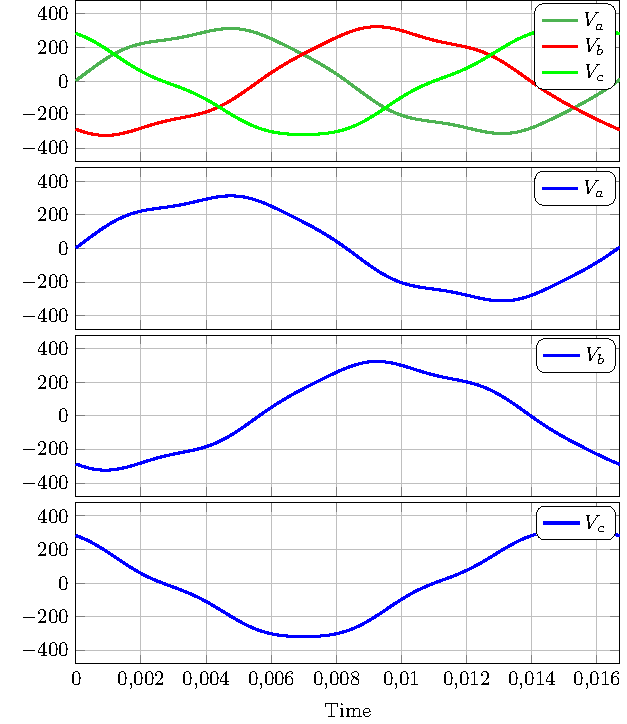
\includegraphics[width=\linewidth]{pictures/ex01}
    \label{fig:ex01}
\fonte{o autor}
\end{figure}

Por exemplo, na \figref{fig:ex01}, tem-se...


\begin{figure}
    \centering
    \caption{Exemplo de aquisição}
    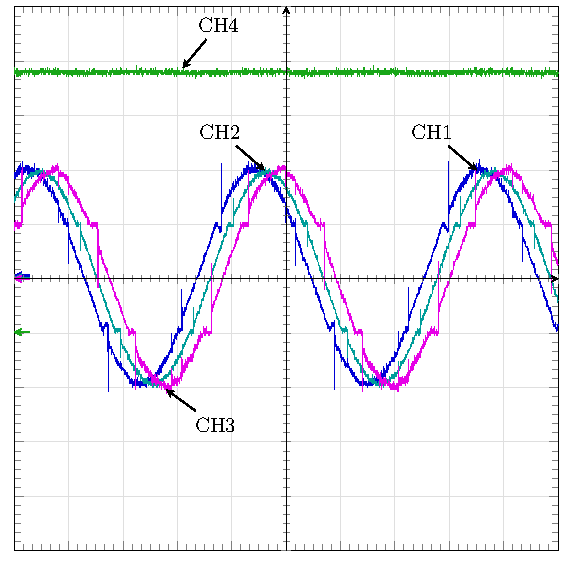
\includegraphics[width=0.9\linewidth]{pictures/tek0009}
    \label{fig:tek0009}
    \fonte{o autor}
\end{figure}

Este documento e seu código-fonte são exemplos de referência de uso da classe
\textsf{abntex2} e do pacote \textsf{abntex2cite}. O documento
exemplifica a elaboração de trabalho acadêmico (tese, dissertação e outros do
gênero) produzido conforme a ABNT NBR 14724:2011 \emph{Informação e documentação
- Trabalhos acadêmicos - Apresentação}.

A expressão ``Modelo Canônico'' é utilizada para indicar que \abnTeX{} não é
modelo específico de nenhuma universidade ou instituição, mas que implementa tão
somente os requisitos das normas da ABNT. Uma lista completa das normas
observadas pelo \abnTeX{} é apresentada em \textcite{abntex2classe}.

Sinta-se convidado a participar do projeto \abnTeX{}! Acesse o site do projeto em
\url{http://abntex2.googlecode.com/}. Também fique livre para conhecer,
estudar, alterar e redistribuir o trabalho do \abnTeX{}, desde que os arquivos
modificados tenham seus nomes alterados e que os créditos sejam dados aos
autores originais, nos termos da ``The \LaTeX{} Project Public
License''\footnote{\url{http://www.latex-project.org/lppl.txt}}.

Encorajamos que sejam realizadas customizações específicas deste exemplo para
universidades e outras instituições --- como capas, folha de aprovação, etc.
Porém, recomendamos que ao invés de se alterar diretamente os arquivos do
\abnTeX{}, distribua-se arquivos com as respectivas customizações.
Isso permite que futuras versões do \abnTeX{}~não se tornem automaticamente
incompatíveis com as customizações promovidas. Consulte
\textcite{abntex2-wiki-como-customizar} par mais informações.

Este documento deve ser utilizado como complemento dos manuais do \abnTeX{}
\cite{abntex2classe,abntex2cite,abntex2cite-alf} e da classe \textsf{memoir}
\cite{memoir}.

Esperamos, sinceramente, que o \abnTeX{} aprimore a qualidade do trabalho que
você produzirá, de modo que o principal esforço seja concentrado no principal:
na contribuição científica.

Equipe \abnTeX{}

Lauro César Araujo

\section{Teste}
\subsection{Teste}
\subsubsection{Teste}
\subsubsubsection{Teste}






    % Capitulo com exemplos de comandos inseridos de arquivo externo
    %% chapters/chapter_1.tex
%%
%% Copyright 2017 Evandro Coan
%% Copyright 2012-2014 by abnTeX2 group at http://abntex2.googlecode.com/
%%
%% This work may be distributed and/or modified under the
%% conditions of the LaTeX Project Public License, either version 1.3
%% of this license or (at your option) any later version.
%% The latest version of this license is in
%%   http://www.latex-project.org/lppl.txt
%% and version 1.3 or later is part of all distributions of LaTeX
%% version 2005/12/01 or later.
%%
%% This work has the LPPL maintenance status `maintained'.
%%
%% The Current Maintainer of this work is the Evandro Coan.
%%
%% The last Maintainer of this work was the abnTeX2 team, led
%% by Lauro César Araujo. Further information are available on
%% https://www.abntex.net.br/
%%
%% This work consists of a bunch of files. But originally there were 2 files
%% which are renamed as follows:
%% Deleted the `abntex2-modelo-img-marca.pdf`
%% Renamed the `abntex2-modelo-include-comandos.tex, v-1.9.2 laurocesar` to `chapters/chapter_1.tex`
%%
% ---
% Este capítulo, utilizado por diferentes exemplos do abnTeX2, ilustra o uso de
% comandos do abnTeX2 e de LaTeX.
% ---

% The \phantomsection command is needed to create a link to a place in the document that is not a
% figure, equation, table, section, subsection, chapter, etc.
%
% When do I need to invoke \phantomsection?
% https://tex.stackexchange.com/questions/44088/when-do-i-need-to-invoke-phantomsection
\phantomsection


% Is it possible to keep my translation together with original text?
% https://tex.stackexchange.com/questions/5076/is-it-possible-to-keep-my-translation-together-with-original-text
\chapter[\lang{Abbreviation for the Table of Contents}{Abreviação para o Sumário}]
{
    \lang
    {Long title to present in the chapter, Axioms, Theorems, Postulates, corollaries, lemmas}
    {Longo título apresentar no capítulo, Axiomas, Teoremas, Postulados, corolários, lemas}
}

\label{cap_exemplos}


\begin{flushright}
    \englishword{ }
\end{flushright}


% \newpage

% Multiple-language document - babel - selectlanguage vs begin/end{otherlanguage}
% https://tex.stackexchange.com/questions/36526/multiple-language-document-babel-selectlanguage-vs-begin-endotherlanguage
\begin{otherlanguage*}{brazil}



\section{Axiomas ou postulados}

Na lógica tradicional, um axioma ou postulado é uma sentença ou proposição que não é provada ou demonstrada e é considerada como óbvia ou como um consenso inicial necessário para a construção ou aceitação de uma teoria. Por essa razão, é aceito como verdade e serve como ponto inicial para dedução e inferências de outras verdades (dependentes de teoria).


Na matemática, um axioma é uma hipótese inicial de qual outros enunciados são logicamente derivados. Pode ser uma sentença, uma proposição, um enunciado ou uma regra que permite a construção de um sistema formal. Diferentemente de teoremas, axiomas não podem ser derivados por princípios de dedução e nem são demonstráveis por derivações formais, simplesmente porque eles são hipóteses iniciais. Isto é, não há mais nada a partir do que eles seguem logicamente (em caso contrário eles seriam chamados teoremas). Em muitos contextos, "axioma", "postulado" e "hipótese" são usados como sinônimos.


\begin{axioma}[Axioma de Igualdade]
Supondo $\mathfrak{L}$, uma linguagem de primeira ordem. para cada variável $x$, a fórmula $x = x$ é universalmente válida.
\end{axioma}


\begin{postulado}[Postulado de Igualdade]
    Supondo $\mathfrak{L}$, uma linguagem de primeira ordem. para cada variável $x$, a fórmula $x = x$ é universalmente válida.
\end{postulado}


\section{Teorema}


Na matemática, um teorema é uma afirmação que pode ser provada como verdadeira através de outras afirmações já demonstradas, como outros teoremas, juntamente com afirmações anteriormente aceitas, como axiomas. Prova é o processo de mostrar que um teorema está correto. O termo teorema foi introduzido por Euclides, em Elementos, para significar "afirmação que pode ser provada". Em grego, originalmente significava "espetáculo" ou "festa". Atualmente, é mais comum deixar o termo "teorema" apenas para certas afirmações que podem ser provadas e de grande "importância matemática", o que torna a definição um tanto subjetiva.

\begin{teorema}[Teorema de Pitágoras]
    Em qualquer triângulo retângulo, o quadrado do comprimento da hipotenusa é igual à soma dos quadrados dos comprimentos dos catetos.
\end{teorema}


\begin{proposicao}
Em qualquer proposição a hipótese é considerada verdadeira.
\end{proposicao}
\subsection{Terminologia}



Usualmente deixa-se o termo ``teorema'' apenas para as afirmações que podem ser provadas de grande importância. Assim, são dados outros nomes para os outros tipos dessas afirmações:

\begin{description}
    \item[Proposição:] Uma Proposição é uma sentença não associada a algum outro teorema, de simples prova e de importância matemática menor.
    \item[Lema:] Um Lema é um ``pré-teorema'', um teorema que serve para ajudar na prova de outro teorema maior. A distinção entre teoremas e lemas é um tanto quanto arbitrária, uma vez que grandes resultados são usados para provar outros. Por exemplo, o Lema de Gauss e o Lema de Zorn são muito interessantes de per se, e muitos autores os denominam de Lemas, mesmo que não os usem para provar alguma outra coisa.
    \item[Corolário:] Um Corolário é uma consequência direta de outro teorema ou de uma definição, muitas vezes tendo suas demonstrações omitidas, por serem simples.
\end{description}


\begin{corolario}
    Em qualquer triângulo retângulo, a hipotenusa é maior que qualquer um dos catetos, mas menor que a soma deles.
\end{corolario}

Alguns outros termos também são usados, por mais que raros e com definição menos rigorosa, basicamente sendo usadas quando não se quer usar a a palavra ``teorema'':

Regra.
Lei, que também pode se referir a axiomas, regras de dedução e a distribuições de Probabilidade.
Princípio.
Algoritmo (como em Algoritmo da Divisão), muito raro e diferente do conceito com o mesmo nome que é um dos estudos centrais da Ciência da Computação.
Paradoxo, usado quando a afirmação vai aparentemente de encontro com alguma outra verdade ou com alguma noção intuitiva. Entretanto, tal termo também pode ser usado para afirmações falsas que aparentem ser verdadeiras em um primeiro momento.

Alguns teoremas continuam a ser chamados de Conjecturas logo após serem provados (por exemplo, a Conjectura de Poincaré). O termo conjectura é usado para afirmações que não se sabe se são verdadeiras, e que acredita-se que são verdadeiras, mas nunca ninguém conseguiu prová-las nem negá-las (às vezes conjecturas são chamadas de hipóteses (como em Hipótese de Riemann), obviamente, num sentido diferente do aqui já descrito).


\subsection{Conjectura ou hipótese}

Uma conjectura é uma ideia, fórmula ou frase, a qual não foi provada ser verdadeira, baseada em suposições ou ideias com fundamento não verificado. As conjecturas utilizadas como prova de resultados matemáticos recebem o nome de hipóteses.



\begin{conjectura}[Conjectura dos primos gêmeos]
Existem infinitos números primos gêmeos.
\end{conjectura}

Um par de primos é chamado de primos gêmeos se eles são dois números primos $p$, $q$ tais que $q = p + 2$.



\subsection{Lema}

    Na Matemática, um lema é um teorema que é usado como um passo intermediário para atingir um resultado maior, provado em outro teorema. Normalmente o lema tem pouca serventia além de servir ao propósito do teorema que o utiliza, mas isto não é uma regra, e a classificação entre lemas e teoremas é arbitrária\footnote{Wikipédia}.


\begin{lema}
    Given two line segments whose lengths are $a$ and $b$ respectively there is a
    real number $r$ such that $b=ra$.
\end{lema}



Unnumbered theorem-like environments are also possible.

\begin{observacao}
    This statement is true, I guess.
\end{observacao}

And the next is a somewhat informal definition


\begin{definicao}[Fibration]
    A fibration is a mapping between two topological spaces that has the homotopy lifting property for every space $X$.
\end{definicao}

\begin{exemplo}[Fibration]
    A fibration is a mapping between two topological spaces that has the homotopy lifting property for every space $X$.
\end{exemplo}


\begin{exercicio}
    Este é um exercício

\end{exercicio}

\begin{exercicio}
    Mais um exercício para vocês...

\end{exercicio}


\begin{condicao}[Fibration]
    A fibration is a mapping between two topological spaces that has the homotopy lifting property for every space $X$.
\end{condicao}
Theorem styles

\begin{description}
    \item[definition] boldface title, romand body. Commonly used in definitions, conditions, problems and examples.
\item[plain] boldface title, italicized body. Commonly used in theorems, lemmas, corollaries, propositions and conjectures.
\item[remark] italicized title, romman body. Commonly used in remarks, notes, annotations, claims, cases, acknowledgments and conclusions.
\end{description}


\section{Rotação de equações}

trecho de código para rotacionar e reduzir a fonte de equações.

\begin{verbatim}
\begin{sideways}%
  \parbox{1\textheight}{%
      \begin{tiny}
          \begin{equation}

          \end{equation}
      \end{tiny}}
\end{sideways}
\end{verbatim}


Segue um exemplo de rotação de páginas: \newpage

\begin{sideways}%
    \parbox{1\textheight}{%
        \begin{tiny}
\begin{equation}
\left[ {{L_{sr}}} \right] = \left[ {\begin{array}{*{20}{c}}
    {\cos \left( \theta  \right)}&{\cos \left( {\theta  - 8\alpha } \right)}&{\cos \left( {\theta  - 7\alpha } \right)}&{\cos \left( {\theta  - 6\alpha } \right)}&{\cos \left( {\theta  - 5\alpha } \right)}&{\cos \left( {\theta  - 4\alpha } \right)}&{\cos \left( {\theta  - 3\alpha } \right)}&{\cos \left( {\theta  - 2\alpha } \right)}&{\cos \left( {\theta  - \alpha } \right)}\\
    {\cos \left( {\theta  - \alpha } \right)}&{\cos \left( \theta  \right)}&{\cos \left( {\theta  - 8\alpha } \right)}&{\cos \left( {\theta  - 7\alpha } \right)}&{\cos \left( {\theta  - 6\alpha } \right)}&{\cos \left( {\theta  - 5\alpha } \right)}&{\cos \left( {\theta  - 4\alpha } \right)}&{\cos \left( {\theta  - 3\alpha } \right)}&{\cos \left( {\theta  - 2\alpha } \right)}\\
    {\cos \left( {\theta  - 2\alpha } \right)}&{\cos \left( {\theta  - \alpha } \right)}&{\cos \left( \theta  \right)}&{\cos \left( {\theta  - 8\alpha } \right)}&{\cos \left( {\theta  - 7\alpha } \right)}&{\cos \left( {\theta  - 6\alpha } \right)}&{\cos \left( {\theta  - 5\alpha } \right)}&{\cos \left( {\theta  - 4\alpha } \right)}&{\cos \left( {\theta  - 3\alpha } \right)}\\
    {\cos \left( {\theta  - 3\alpha } \right)}&{\cos \left( {\theta  - 2\alpha } \right)}&{\cos \left( {\theta  - \alpha } \right)}&{\cos \left( \theta  \right)}&{\cos \left( {\theta  - 8\alpha } \right)}&{\cos \left( {\theta  - 7\alpha } \right)}&{\cos \left( {\theta  - 6\alpha } \right)}&{\cos \left( {\theta  - 5\alpha } \right)}&{\cos \left( {\theta  - 4\alpha } \right)}\\
    {\cos \left( {\theta  - 4\alpha } \right)}&{\cos \left( {\theta  - 3\alpha } \right)}&{\cos \left( {\theta  - 2\alpha } \right)}&{\cos \left( {\theta  - \alpha } \right)}&{\cos \left( \theta  \right)}&{\cos \left( {\theta  - 8\alpha } \right)}&{\cos \left( {\theta  - 7\alpha } \right)}&{\cos \left( {\theta  - 6\alpha } \right)}&{\cos \left( {\theta  - 5\alpha } \right)}\\
    {\cos \left( {\theta  - 5\alpha } \right)}&{\cos \left( {\theta  - 4\alpha } \right)}&{\cos \left( {\theta  - 3\alpha } \right)}&{\cos \left( {\theta  - 2\alpha } \right)}&{\cos \left( {\theta  - \alpha } \right)}&{\cos \left( \theta  \right)}&{\cos \left( {\theta  - 8\alpha } \right)}&{\cos \left( {\theta  - 7\alpha } \right)}&{\cos \left( {\theta  - 6\alpha } \right)}\\
    {\cos \left( {\theta  - 6\alpha } \right)}&{\cos \left( {\theta  - 5\alpha } \right)}&{\cos \left( {\theta  - 4\alpha } \right)}&{\cos \left( {\theta  - 3\alpha } \right)}&{\cos \left( {\theta  - 2\alpha } \right)}&{\cos \left( {\theta  - \alpha } \right)}&{\cos \left( \theta  \right)}&{\cos \left( {\theta  - 8\alpha } \right)}&{\cos \left( {\theta  - 7\alpha } \right)}\\
    {\cos \left( {\theta  - 7\alpha } \right)}&{\cos \left( {\theta  - 6\alpha } \right)}&{\cos \left( {\theta  - 5\alpha } \right)}&{\cos \left( {\theta  - 4\alpha } \right)}&{\cos \left( {\theta  - 3\alpha } \right)}&{\cos \left( {\theta  - 2\alpha } \right)}&{\cos \left( {\theta  - \alpha } \right)}&{\cos \left( \theta  \right)}&{\cos \left( {\theta  - 8\alpha } \right)}\\
    {\cos \left( {\theta  - 8\alpha } \right)}&{\cos \left( {\theta  - 7\alpha } \right)}&{\cos \left( {\theta  - 6\alpha } \right)}&{\cos \left( {\theta  - 5\alpha } \right)}&{\cos \left( {\theta  - 4\alpha } \right)}&{\cos \left( {\theta  - 3\alpha } \right)}&{\cos \left( {\theta  - 2\alpha } \right)}&{\cos \left( {\theta  - \alpha } \right)}&{\cos \left( \theta  \right)}
    \end{array}} \right]
\end{equation}
\end{tiny}
}
\end{sideways}


\begin{landscape}

Outra forma é utilizar o pacote pdflscape

% Reducing font size in equation
% https://tex.stackexchange.com/questions/60453/reducing-font-size-in-equation
\tiny
\begin{equation}
\left[ {{L_{sr}}} \right] = \left[ {\begin{array}{*{20}{c}}
    {\cos \left( \theta  \right)}&{\cos \left( {\theta  - 8\alpha } \right)}&{\cos \left( {\theta  - 7\alpha } \right)}&{\cos \left( {\theta  - 6\alpha } \right)}&{\cos \left( {\theta  - 5\alpha } \right)}&{\cos \left( {\theta  - 4\alpha } \right)}&{\cos \left( {\theta  - 3\alpha } \right)}&{\cos \left( {\theta  - 2\alpha } \right)}&{\cos \left( {\theta  - \alpha } \right)}\\
    {\cos \left( {\theta  - \alpha } \right)}&{\cos \left( \theta  \right)}&{\cos \left( {\theta  - 8\alpha } \right)}&{\cos \left( {\theta  - 7\alpha } \right)}&{\cos \left( {\theta  - 6\alpha } \right)}&{\cos \left( {\theta  - 5\alpha } \right)}&{\cos \left( {\theta  - 4\alpha } \right)}&{\cos \left( {\theta  - 3\alpha } \right)}&{\cos \left( {\theta  - 2\alpha } \right)}\\
    {\cos \left( {\theta  - 2\alpha } \right)}&{\cos \left( {\theta  - \alpha } \right)}&{\cos \left( \theta  \right)}&{\cos \left( {\theta  - 8\alpha } \right)}&{\cos \left( {\theta  - 7\alpha } \right)}&{\cos \left( {\theta  - 6\alpha } \right)}&{\cos \left( {\theta  - 5\alpha } \right)}&{\cos \left( {\theta  - 4\alpha } \right)}&{\cos \left( {\theta  - 3\alpha } \right)}\\
    {\cos \left( {\theta  - 3\alpha } \right)}&{\cos \left( {\theta  - 2\alpha } \right)}&{\cos \left( {\theta  - \alpha } \right)}&{\cos \left( \theta  \right)}&{\cos \left( {\theta  - 8\alpha } \right)}&{\cos \left( {\theta  - 7\alpha } \right)}&{\cos \left( {\theta  - 6\alpha } \right)}&{\cos \left( {\theta  - 5\alpha } \right)}&{\cos \left( {\theta  - 4\alpha } \right)}\\
    {\cos \left( {\theta  - 4\alpha } \right)}&{\cos \left( {\theta  - 3\alpha } \right)}&{\cos \left( {\theta  - 2\alpha } \right)}&{\cos \left( {\theta  - \alpha } \right)}&{\cos \left( \theta  \right)}&{\cos \left( {\theta  - 8\alpha } \right)}&{\cos \left( {\theta  - 7\alpha } \right)}&{\cos \left( {\theta  - 6\alpha } \right)}&{\cos \left( {\theta  - 5\alpha } \right)}\\
    {\cos \left( {\theta  - 5\alpha } \right)}&{\cos \left( {\theta  - 4\alpha } \right)}&{\cos \left( {\theta  - 3\alpha } \right)}&{\cos \left( {\theta  - 2\alpha } \right)}&{\cos \left( {\theta  - \alpha } \right)}&{\cos \left( \theta  \right)}&{\cos \left( {\theta  - 8\alpha } \right)}&{\cos \left( {\theta  - 7\alpha } \right)}&{\cos \left( {\theta  - 6\alpha } \right)}\\
    {\cos \left( {\theta  - 6\alpha } \right)}&{\cos \left( {\theta  - 5\alpha } \right)}&{\cos \left( {\theta  - 4\alpha } \right)}&{\cos \left( {\theta  - 3\alpha } \right)}&{\cos \left( {\theta  - 2\alpha } \right)}&{\cos \left( {\theta  - \alpha } \right)}&{\cos \left( \theta  \right)}&{\cos \left( {\theta  - 8\alpha } \right)}&{\cos \left( {\theta  - 7\alpha } \right)}\\
    {\cos \left( {\theta  - 7\alpha } \right)}&{\cos \left( {\theta  - 6\alpha } \right)}&{\cos \left( {\theta  - 5\alpha } \right)}&{\cos \left( {\theta  - 4\alpha } \right)}&{\cos \left( {\theta  - 3\alpha } \right)}&{\cos \left( {\theta  - 2\alpha } \right)}&{\cos \left( {\theta  - \alpha } \right)}&{\cos \left( \theta  \right)}&{\cos \left( {\theta  - 8\alpha } \right)}\\
    {\cos \left( {\theta  - 8\alpha } \right)}&{\cos \left( {\theta  - 7\alpha } \right)}&{\cos \left( {\theta  - 6\alpha } \right)}&{\cos \left( {\theta  - 5\alpha } \right)}&{\cos \left( {\theta  - 4\alpha } \right)}&{\cos \left( {\theta  - 3\alpha } \right)}&{\cos \left( {\theta  - 2\alpha } \right)}&{\cos \left( {\theta  - \alpha } \right)}&{\cos \left( \theta  \right)}
    \end{array}} \right]
\end{equation}
\normalsize

\end{landscape}




% ---
\section{Codificação dos arquivos: UTF8}
% ---

 


A codificação de todos os arquivos do \abnTeX{} é \texttt{UTF8}. É necessário que
você utilize a mesma codificação nos documentos que escrever, inclusive nos
arquivos de base bibliográficas |.bib|.

% ---
\section{Citações diretas}
\label{sec-citacao}
% ---

\index{citações!diretas}Utilize o ambiente \texttt{citacao} para incluir
citações diretas com mais de três linhas:

\begin{citacao}
As citações diretas, no texto, com mais de três linhas, devem ser
destacadas com recuo de 4 cm da margem esquerda, com letra menor que a do texto
utilizado e sem as aspas. No caso de documentos datilografados, deve-se
observar apenas o recuo \cite[5.3]{NBR10520:2002}.

 
\end{citacao}

 
Use o ambiente assim:

\begin{lstlisting}[language=tex]
\begin{citacao}
As citações diretas, no texto, com mais de três linhas [...]
deve-se observar apenas o recuo \cite[5.3]{NBR10520:2002}.
\end{citacao}
\end{lstlisting}

 

O ambiente \texttt{citacao} pode receber como parâmetro opcional um nome de
idioma previamente carregado nas opções da classe (\autoref{sec-hifenizacao}). Nesse
caso, o texto da citação é automaticamente escrito em itálico e a hifenização é
ajustada para o idioma selecionado na opção do ambiente. Por exemplo:

\begin{lstlisting}[language=tex]
\begin{citacao}[english]
Text in English language in italic with correct hyphenation.
\end{citacao}
\end{lstlisting}

Tem como resultado:

\begin{citacao}[english]
Text in English language in italic with correct hyphenation.
\end{citacao}

\index{citações!simples}Citações simples, com até três linhas, devem ser
incluídas com aspas. Observe que em \LaTeX{} as aspas iniciais são diferentes das
finais: ``Amor é fogo que arde sem se ver''.

% ---
\section{Notas de rodapé}
% ---

As notas de rodapé são detalhadas pela NBR 14724:2011 na seção 5.2.1\footnote{As
notas devem ser digitadas ou datilografadas dentro das margens, ficando
separadas do texto por um espaço simples de entre as linhas e por filete de 5
cm, a partir da margem esquerda. Devem ser alinhadas, a partir da segunda linha
da mesma nota, abaixo da primeira letra da primeira palavra, de forma a destacar
o expoente, sem espaço entre elas e com fonte menor
\textcite[5.2.1]{NBR14724:2011}.}\footnote{Caso uma série de notas sejam
criadas sequencialmente, o \abnTeX{} instrui o \LaTeX{} para que uma vírgula seja
colocada após cada número do expoente que indica a nota de rodapé no corpo do
texto.}\footnote{Verifique se os números do expoente possuem uma vírgula para
dividi-los no corpo do texto.}.


% ---
\section{Tabelas}
% ---

\index{tabelas}A \autoref{tab-nivinv} é um exemplo de tabela construída em
\LaTeX{}.

\begin{table}[htb]
\caption[Níveis de investigação]{Níveis de investigação.}
\label{tab-nivinv}
\resizebox{\textwidth}{!}{%
\begin{tabular}{p{2.6cm}p{6.0cm}p{2.25cm}p{3.40cm}}
  \toprule
   \textbf{Nível de Investigação} & \textbf{Insumos}  & \textbf{Sistemas de Investigação}  & \textbf{Produtos}  \\
    \midrule
    Meta-nível & Filosofia\index{filosofia} da Ciência  & Epistemologia &
    Paradigma  \\
    Nível do objeto & Paradigmas do metanível e evidências do nível inferior &
    Ciência  & Teorias e modelos \\
    Nível inferior & Modelos e métodos do nível do objeto e problemas do nível inferior & Prática & Solução de problemas  \\
   \bottomrule
\end{tabular}
}
\fonte{\textcite{van86}}
\end{table}


Já a \autoref{tabela-ibge} apresenta uma tabela criada conforme o padrão do
\textcite{ibge1993} requerido pelas normas da ABNT para documentos técnicos e
acadêmicos.


\begin{table}[htb]
\IBGEtab{%
  \caption{Um Exemplo de tabela alinhada que pode ser longa
  ou curta, conforme padrão IBGE.}%
  \label{tabela-ibge}
}{%
  \begin{tabular}{ccc}
  \toprule
   \textbf{Nome} & \textbf{Nascimento} & \textbf{Documento} \\
  \midrule 
   Maria da Silva & 11/11/1111 & 111.111.111-11 \\
  \midrule
   João Souza & 11/11/2111 & 211.111.111-11 \\
  \midrule
   Laura Vicuña & 05/04/1891 & 3111.111.111-11 \\
  \bottomrule
\end{tabular}%
}{%
  \fonte{Produzido pelos autores.}%
  \nota{Esta é uma nota, que diz que os dados são baseados na
  regressão linear.}%
  \nota[Anotações]{Uma anotação adicional, que pode ser seguida de várias
  outras.}%
  }
\end{table}



% What does [t] and [ht] mean?
% https://tex.stackexchange.com/questions/8652/what-does-t-and-ht-mean
\begin{table}[!ht]
    \caption{Exemplo de tabela utilizando o pacote \emph{siunitx} e \emph{resizebox}.}
    \label{tab:SimulationResults}
    \centering
    \resizebox{\linewidth}{!}{%
        \begin{tabular}{cc|cc|cc} \toprule
            \multicolumn{2}{l}{\textbf{Fase A} } & \multicolumn{2}{l}{\textbf{Fase B}}
            & \multicolumn{2}{l}{\textbf{Fase C}} \\ \hline
            Parâmetro       & Valor       & Parâmetro        & Valor        & Parâmetro         & Valor            \\\hline
            $I_{La1}$&$\SI{2.9082866e+000}{\A}$&  $I_{Lb1}$&$\SI{3.3878432e+000}{\A}$& $I_{Lc1}$&$\SI{3.0354175e+000}{\A}$ \\
            $I_{La2}$&$\SI{2.9083278e+000}{\A}$&  $I_{Lb2}$&$\SI{3.3935604e+000}{\A}$& $I_{Lc2}$&$\SI{3.0238770e+000}{\A}$ \\
            $I_{La3}$&$\SI{2.9057255e+000}{\A}$&  $I_{Lb3}$&$\SI{3.3936165e+000}{\A}$& $I_{Lc3}$&$\SI{3.0252536e+000}{\A}$ \\
            $P_{a1}$& $\SI{625.50259e+00}{\W}$&  $P_{b1}$& $\SI{724.85424e+00}{\W}$& $P_{c1}$& $\SI{662.06883e+00}{\W}$ \\
            $P_{a2}$& $\SI{625.31121e+00}{\W}$&  $P_{b2}$& $\SI{725.62100e+00}{\W}$& $P_{c2}$& $\SI{660.36375e+00}{\W}$ \\
            $P_{a3}$& $\SI{625.96179e+00 }{\W}$&  $P_{b3}$& $\SI{725.28968e+00}{\W}$& $P_{c3}$& $\SI{660.14426e+00}{\W}$ \\
            $Q_{a1}$& $\SI{36.605745e+00 }{\VA}$&  $Q_{b1}$& $\SI{45.613691e+00}{\VA}$& $Q_{c1}$& $\SI{54.531747e+00}{\VA}$ \\
            $Q_{a2}$& $\SI{19.160357e+00}{\VA}$&  $Q_{b2}$& $\SI{36.608133e+00}{\VA}$& $Q_{c2}$& $\SI{19.939460e+00}{\VA}$ \\
            $Q_{a3}$& $\SI{18.867027e+00}{\VA}$&  $Q_{b3}$& $\SI{47.791169e+00}{\VA}$& $Q_{c3}$& $\SI{13.797842e+00}{\VA}$ \\
            $V_{Ca1}$&$\SI{400.04695e+00}{\V}$&  $V_{Cb1}$&$\SI{400.00862e+00}{\V}$& $V_{Cc1}$&$\SI{400.11656e+00}{\V}$ \\
            $V_{Ca2}$&$\SI{399.93041e+00}{\V}$&  $V_{Cb2}$&$\SI{400.05835e+00}{\V}$& $V_{Cc2}$&$\SI{399.97514e+00}{\V}$ \\
            $V_{Ca3}$&$\SI{400.02312e+00}{\V}$&  $V_{Cb3}$&$\SI{399.93403e+00}{\V}$& $V_{Cc3}$&$\SI{399.90881e+00}{\V}$ \\
            $I_{Ca1}$&$\SI{1.2605228e+000}{\A}$&  $I_{Cb1}$&$\SI{1.4684945e+000}{\A}$& $I_{Cc1}$&$\SI{1.3054048e+000}{\A}$ \\
            $I_{Ca2}$&$\SI{1.2661075e+000}{\A}$&  $I_{Cb2}$&$\SI{1.4720236e+000}{\A}$& $I_{Cc2}$&$\SI{1.3089556e+000}{\A}$ \\
            $I_{Ca3}$&$\SI{1.2598194e+000}{\A}$&  $I_{Cb3}$&$\SI{1.4708279e+000}{\A}$& $I_{Cc3}$&$\SI{1.3017673e+000}{\A}$ \\
            \bottomrule
        \end{tabular}}
\fonte{O autor}
\end{table}




\clearpage
% ---
\section{Figuras}
% ---

\index{figuras}Figuras podem ser criadas diretamente em \LaTeX{},
como o exemplo da \autoref{fig_circulo}.

\begin{figure}[htb]
    \caption{\label{fig_circulo}A delimitação do espaço}
    \begin{center}
        \setlength{\unitlength}{5cm}
        \begin{picture}(1,1)
        \put(0,0){\line(0,1){1}}
        \put(0,0){\line(1,0){1}}
        \put(0,0){\line(1,1){1}}
        \put(0,0){\line(1,2){.5}}
        \put(0,0){\line(1,3){.3333}}
        \put(0,0){\line(1,4){.25}}
        \put(0,0){\line(1,5){.2}}
        \put(0,0){\line(1,6){.1667}}
        \put(0,0){\line(2,1){1}}
        \put(0,0){\line(2,3){.6667}}
        \put(0,0){\line(2,5){.4}}
        \put(0,0){\line(3,1){1}}
        \put(0,0){\line(3,2){1}}
        \put(0,0){\line(3,4){.75}}
        \put(0,0){\line(3,5){.6}}
        \put(0,0){\line(4,1){1}}
        \put(0,0){\line(4,3){1}}
        \put(0,0){\line(4,5){.8}}
        \put(0,0){\line(5,1){1}}
        \put(0,0){\line(5,2){1}}
        \put(0,0){\line(5,3){1}}
        \put(0,0){\line(5,4){1}}
        \put(0,0){\line(5,6){.8333}}
        \put(0,0){\line(6,1){1}}
        \put(0,0){\line(6,5){1}}
        \end{picture}
    \end{center}
    \fonte{os autores}
\end{figure}






Ou então figuras podem ser incorporadas de arquivos externos, como é o caso da
\autoref{fig_grafico}. Se a figura que ser incluída se tratar de um diagrama, um
gráfico ou uma ilustração que você mesmo produza, priorize o uso de imagens
vetoriais no formato PDF. Com isso, o tamanho do arquivo final do trabalho será
menor, e as imagens terão uma apresentação melhor, principalmente quando
impressas, uma vez que imagens vetorias são perfeitamente escaláveis para
qualquer dimensão. Nesse caso, se for utilizar o Microsoft Excel para produzir
gráficos, ou o Microsoft Word para produzir ilustrações, exporte-os como PDF e
os incorpore ao documento conforme o exemplo abaixo. No entanto, para manter a
coerência no uso de software livre (já que você está usando \LaTeX{} e \abnTeX{}),
teste a ferramenta \textsf{InkScape}\index{InkScape}
(\url{http://inkscape.org/}). Ela é uma excelente opção de código-livre para
produzir ilustrações vetoriais, similar ao CorelDraw\index{CorelDraw} ou ao Adobe
Illustrator\index{Adobe Illustrator}. De todo modo, caso não seja possível
utilizar arquivos de imagens como PDF, utilize qualquer outro formato, como
JPEG, GIF, BMP, etc. Nesse caso, você pode tentar aprimorar as imagens
incorporadas com o software livre \textsf{Gimp}\index{Gimp}
(\url{http://www.gimp.org/}). Ele é uma alternativa livre ao Adobe
Photoshop\index{Adobe Photoshop}.

\begin{figure}[htb]
    \caption{\label{fig_grafico}Gráfico produzido em Excel e salvo como PDF}
    \begin{center}
        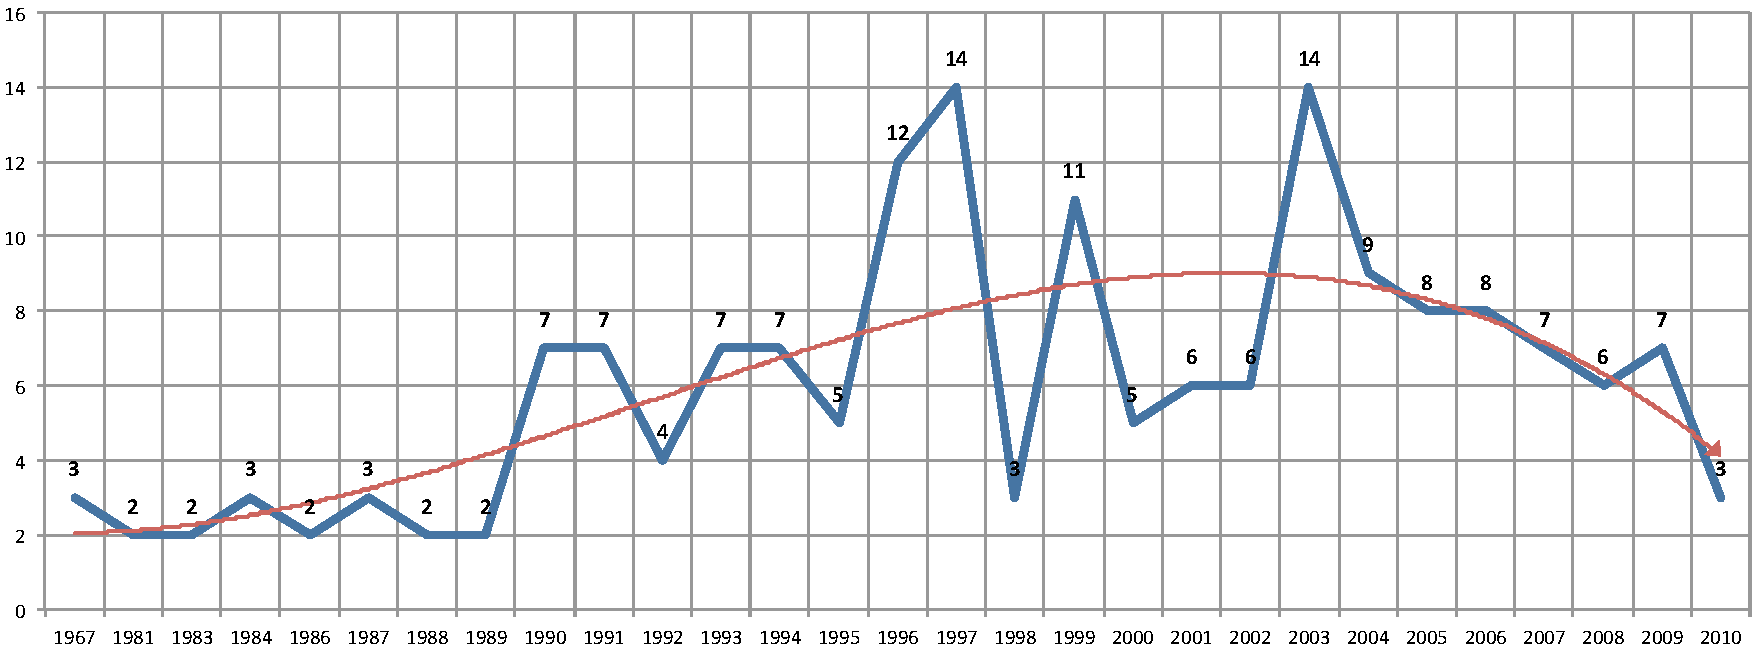
\includegraphics[scale=0.35]{pictures/abntex2-modelo-img-grafico.pdf}
    \end{center}
    \fonte{\textcite[p. 24]{araujo2012}}
\end{figure}

% ---
\subsection{Figuras em minipages}
% ---

Minipages são usadas para inserir textos ou outros elementos em quadros
com tamanhos e posições controladas. Veja o exemplo da
\autoref{fig_minipage_imagem1} e da \autoref{fig_minipage_grafico2}.

\begin{figure}[htb]
\label{teste}
\centering
 \begin{minipage}{0.49\textwidth}
   \centering
   \caption{Imagem 1 da minipage} \label{fig_minipage_imagem1}
   
\includegraphics[width=\textwidth]{pictures/abntex2-modelo-img-marca.pdf}
   \fonte{Produzido pelos autores}
 \end{minipage}
 \hfill
 \begin{minipage}{0.49\textwidth}
   \centering
   \caption{Gráfico 2 da minipage} \label{fig_minipage_grafico2}
   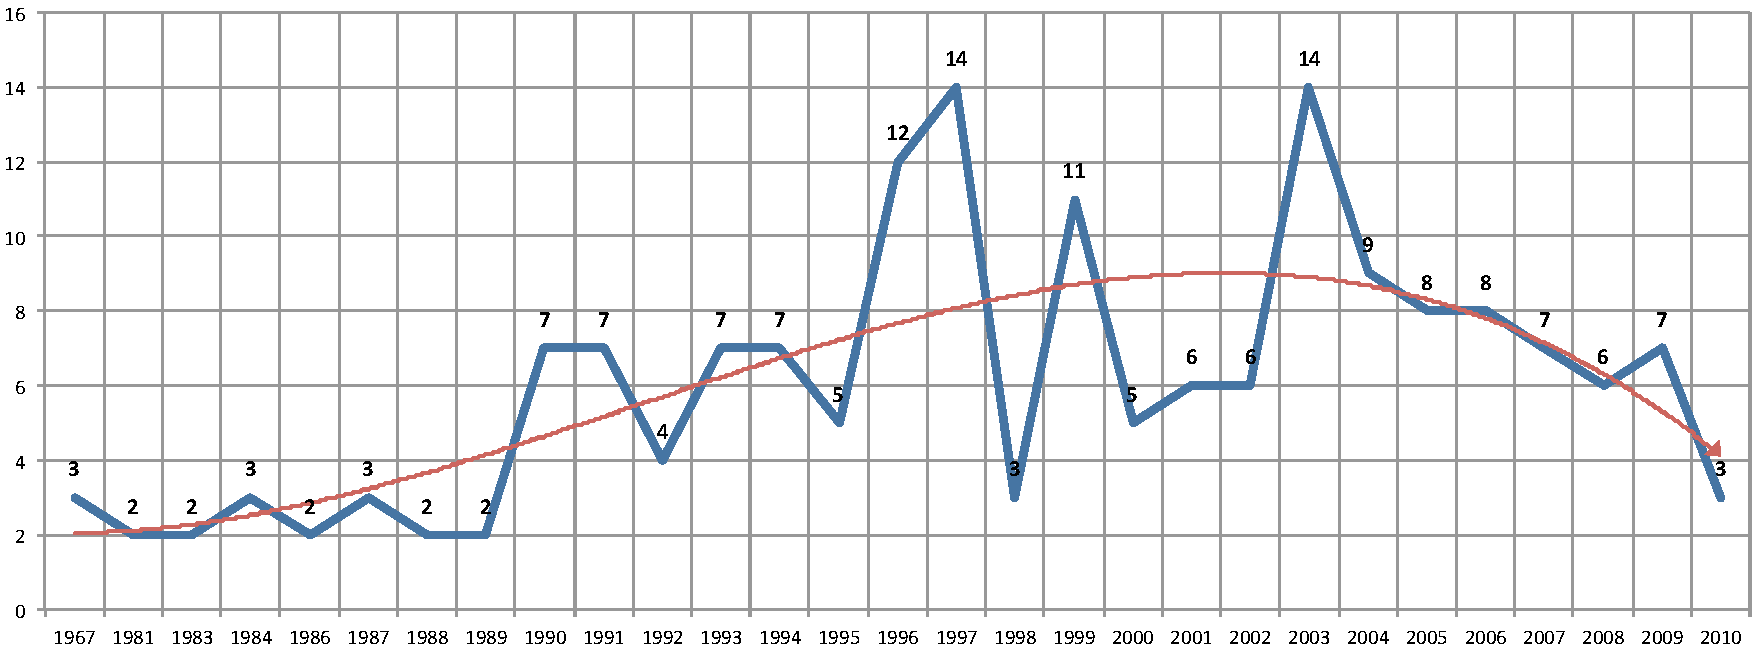
\includegraphics[width=\textwidth]{pictures/abntex2-modelo-img-grafico.pdf}
   \fonte{\textcite[p. 24]{araujo2012}}
 \end{minipage}
\end{figure}



Observe que, segundo a \textcite[seções 4.2.1.10 e 5.8]{NBR14724:2011}, as
ilustrações devem sempre ter numeração contínua e única em todo o documento:

\begin{citacao}
Qualquer que seja o tipo de ilustração, sua identificação aparece na parte
superior, precedida da palavra designativa (desenho, esquema, fluxograma,
fotografia, gráfico, mapa, organograma, planta, quadro, retrato, figura,
imagem, entre outros), seguida de seu número de ordem de ocorrência no texto,
em algarismos arábicos, travessão e do respectivo título. Após a ilustração, na
parte inferior, indicar a fonte consultada (elemento obrigatório, mesmo que
seja produção do próprio autor), legenda, notas e outras informações
necessárias à sua compreensão (se houver). A ilustração deve ser citada no
texto e inserida o mais próximo possível do trecho a que se
refere. \cite[seções 5.8]{NBR14724:2011}
\end{citacao}

% ---
\section{Quadros}
% ---

Depois de definir o ambiente \texttt{quadro} podemos ter um quadro:

\begin{quadro}
\caption{\label{quad:quadro_modelo1}Legenda do primeiro quadro.}
\centering
\begin{tabular}{|c|}
\hline
Este é o conteúdo do primeiro quadro.\\
\hline
\end{tabular}
\fonte{Teste.}
\end{quadro}


Além do \autoref{quad:quadro_modelo1}, também é possível especificar outra ordem de posicionamento como [htb]:

\begin{quadro}[htb]
\centering
\caption{\label{quad:quadro_modelo2}Legenda do segundo quadro.}
\begin{tabular}{|c|}
\hline
Este é o conteúdo do segundo quadro.\\
\hline
\end{tabular}
\fonte{O autor.}
\end{quadro}



% ---
\section{Expressões matemáticas}
% ---

\index{expressões matemáticas} Use o ambiente \texttt{equation} para escrever
expressões matemáticas numeradas:

\begin{equation}
  \forall x \in X, \quad \exists \: y \leq \epsilon
\end{equation}

Escreva expressões matemáticas entre \$ e \$, como em

 $\lim_{x \to \infty}
\exp(-x) = 0 $, para que fiquem na mesma linha.

Também é possível usar colchetes para indicar o início de uma expressão
matemática que não é numerada.

\[
\left|\sum_{i=1}^n a_ib_i\right|
\le
\left(\sum_{i=1}^n a_i^2\right)^{1/2}
\left(\sum_{i=1}^n b_i^2\right)^{1/2}
\]

Consulte mais informações sobre expressões matemáticas em
\url{https://code.google.com/p/abntex2/wiki/Referencias}.






% ---
\section{Enumerações: alíneas e subalíneas}
% ---

\index{alíneas}\index{subalíneas}\index{incisos}Quando for necessário enumerar
os diversos assuntos de uma seção que não possua título, esta deve ser
subdividida em alíneas \cite[4.2]{NBR6024:2012}:

\begin{alineas}

  \item os diversos assuntos que não possuam título próprio, dentro de uma mesma
  seção, devem ser subdivididos em alíneas;

  \item o texto que antecede as alíneas termina em dois pontos;
  \item as alíneas devem ser indicadas alfabeticamente, em letra minúscula,
  seguida de parêntese. Utilizam-se letras dobradas, quando esgotadas as
  letras do alfabeto;

  \item as letras indicativas das alíneas devem apresentar recuo em relação à
  margem esquerda;

  \item o texto da alínea deve começar por letra minúscula e terminar em
  ponto-e-vírgula, exceto a última alínea que termina em ponto final;

  \item o texto da alínea deve terminar em dois pontos, se houver subalínea;

  \item a segunda e as seguintes linhas do texto da alínea começa sob a
  primeira letra do texto da própria alínea;

  \item subalíneas \cite[4.3]{NBR6024:2012} devem ser conforme as alíneas a
  seguir:

  \begin{alineas}
     \item as subalíneas devem começar por travessão seguido de espaço;

     \item as subalíneas devem apresentar recuo em relação à alínea;

     \item o texto da subalínea deve começar por letra minúscula e terminar em
     ponto-e-vírgula. A última subalínea deve terminar em ponto final, se não
     houver alínea subsequente;

     \item a segunda e as seguintes linhas do texto da subalínea começam sob a
     primeira letra do texto da própria subalínea.
  \end{alineas}

  \item no \abnTeX{} estão disponíveis os ambientes \texttt{incisos} e
  \texttt{subalineas}, que em suma são o mesmo que se criar outro nível de
  \texttt{alineas}, como nos exemplos à seguir:

  \begin{incisos}
    \item \textit{Um novo inciso em itálico};
  \end{incisos}

  \item Alínea em \textbf{negrito}:

  \begin{subalineas}
    \item \textit{Uma subalínea em itálico};
    \item \underline{\textit{Uma subalínea em itálico e sublinhado}};
  \end{subalineas}

  \item Última alínea com \emph{ênfase}.

\end{alineas}

% ---
\section{Espaçamento entre parágrafos e linhas}
% ---

\index{espaçamento!dos parágrafos}O tamanho do parágrafo, espaço entre a margem
e o início da frase do parágrafo, é definido por:

\begin{lstlisting}[language=tex]
   \setlength{\parindent}{1.3cm}
\end{lstlisting}

\index{espaçamento!do primeiro parágrafo}Por padrão, não há espaçamento no
primeiro parágrafo de cada início de divisão do documento
(\autoref{sec-divisoes}). Porém, você pode definir que o primeiro parágrafo
também seja indentado, como é o caso deste documento. Para isso, apenas inclua o
pacote \textsf{indentfirst} no preâmbulo do documento:

\begin{lstlisting}[language=tex]
   \usepackage{indentfirst}      % Indenta o primeiro parágrafo de cada seção.
\end{lstlisting}

\index{espaçamento!entre os parágrafos}O espaçamento entre um parágrafo e outro
pode ser controlado por meio do comando:

\begin{verbnobox}[\small]
  \setlength{\parskip}{0.2cm}  % tente também \onelineskip
\end{verbnobox}

\index{espaçamento!entre as linhas}O controle do espaçamento entre linhas é
definido por:

\begin{lstlisting}[language=tex]
  \OnehalfSpacing       % espaçamento um e meio (padrão);
  \DoubleSpacing        % espaçamento duplo
  \SingleSpacing        % espaçamento simples
\end{lstlisting}

Para isso, também estão disponíveis os ambientes:

\begin{lstlisting}[language=tex]
  \begin{SingleSpace} ...\end{SingleSpace}
  \begin{Spacing}{hfactori} ... \end{Spacing}
  \begin{OnehalfSpace} ... \end{OnehalfSpace}
  \begin{OnehalfSpace*} ... \end{OnehalfSpace*}
  \begin{DoubleSpace} ... \end{DoubleSpace}
  \begin{DoubleSpace*} ... \end{DoubleSpace*}
\end{lstlisting}

Para mais informações, consulte \textcite[p. 47-52 e 135]{memoir}.

% ---
\section{Inclusão de código fonte}\label{sec-codeinsert}
% ---

\begin{lstlisting}[caption={Leitura dos dados simulados e conversão para estados topológicos.},label={lst:leituradadossim}]
% Pré definições iniciais
nsub=3;  % Numero de Submódulos
nbits=2*nsub; % Numero de bits necessários para representar os estados
nlevels=2*nsub+1; % Numero total de níveis

% Leitura dos pontos gerados por simulação
time=data(1,:)'; % extrai vetor de tempo
PWM=logical(data(2:end,:))'; % Conversão dos pulsos PWM para estados lógicos

% Cria vetor de string binário com os estados correspondentes
binstates=num2str([PWM(:,1) PWM(:,3) PWM(:,5) PWM(:,7) PWM(:,9) PWM(:,11)]);
state=fi(bin2dec(binstates),0,nbits,0); % Objeto numérico de ponto-fixo

\end{lstlisting}



\begin{lstlisting}[language=Python, caption=Python example]
import numpy as np

def incmatrix(genl1,genl2):
    m = len(genl1)
    n = len(genl2)
    M = None #to become the incidence matrix
    VT = np.zeros((n*m,1), int)  #dummy variable

    #compute the bitwise xor matrix
    M1 = bitxormatrix(genl1)
    M2 = np.triu(bitxormatrix(genl2),1)

    for i in range(m-1):
        for j in range(i+1, m):
            [r,c] = np.where(M2 == M1[i,j])
            for k in range(len(r)):
                VT[(i)*n + r[k]] = 1;
                VT[(i)*n + c[k]] = 1;
                VT[(j)*n + r[k]] = 1;
                VT[(j)*n + c[k]] = 1;

                if M is None:
                    M = np.copy(VT)
                else:
                M = np.concatenate((M, VT), 1)

                VT = np.zeros((n*m,1), int)

    return M
\end{lstlisting}




% ---
\section{Inclusão de outros arquivos}\label{sec-include}
% ---

É uma boa prática dividir o seu documento em diversos arquivos, e não
apenas escrever tudo em um único. Esse recurso foi utilizado neste
documento. Para incluir diferentes arquivos em um arquivo principal,
de modo que cada arquivo incluído fique em uma página diferente, utilize o
comando:

\begin{lstlisting}[language=tex]
   \include{documento-a-ser-incluido}      % sem a extensão .tex
\end{lstlisting}

Para incluir documentos sem quebra de páginas, utilize:

\begin{lstlisting}[language=tex]
   \input{documento-a-ser-incluido}      % sem a extensão .tex
\end{lstlisting}

% ---
\section{Compilar o documento \LaTeX{}}
% ---

 

Geralmente os editores \LaTeX{}, como o
TeXlipse\footnote{\url{http://texlipse.sourceforge.net/}}, o
Texmaker\footnote{\url{http://www.xm1math.net/texmaker/}}, entre outros,
compilam os documentos automaticamente, de modo que você não precisa se
preocupar com isso.

No entanto, você pode compilar os documentos \LaTeX{} usando os seguintes
comandos, que devem ser digitados no \emph{Prompt de Comandos} do Windows ou no
\emph{Terminal} do Mac ou do Linux:

\begin{lstlisting}[language=bash,caption={Você pode compilar os documentos \LaTeX{} usando os seguintes
comandos.},label={lst:compilarLatex}]
   pdflatex ARQUIVO_PRINCIPAL.tex
   bibtex ARQUIVO_PRINCIPAL.aux
   makeindex ARQUIVO_PRINCIPAL.idx
   makeindex ARQUIVO_PRINCIPAL.nlo -s nomencl.ist -o
     ARQUIVO_PRINCIPAL.nls
   pdflatex ARQUIVO_PRINCIPAL.tex
   pdflatex ARQUIVO_PRINCIPAL.tex
\end{lstlisting}

\begin{lstlisting}[language=bash]
a very long and totruous path which you can check to see if it breaks and where at the end of the line
\end{lstlisting}


% ---
\section{Remissões internas}
% ---

Ao nomear a \autoref{tab-nivinv} e a \autoref{fig_circulo}, apresentamos um
exemplo de remissão interna, que também pode ser feita quando indicamos o
\autoref{cap_exemplos}, que tem o nome \emph{\nameref{cap_exemplos}}. O número
do capítulo indicado é \ref{cap_exemplos}, que se inicia à
\autopageref{cap_exemplos}\footnote{O número da página de uma remissão pode ser
obtida também assim:
\pageref{cap_exemplos}.}.
Veja a \autoref{sec-divisoes} para outros exemplos de remissões internas entre
seções, subseções e subsubseções.

O código usado para produzir o texto desta seção é:

\begin{lstlisting}[language=TeX, caption=TeX example]
Ao nomear a \autoref{tab-nivinv} e a \autoref{fig_circulo}, apresentamos um
exemplo de remissão interna, que também pode ser feita quando indicamos o
\autoref{cap_exemplos}, que tem o nome \emph{\nameref{cap_exemplos}}. O número
do capítulo indicado é \ref{cap_exemplos}, que se inicia à
\autopageref{cap_exemplos}\footnote{O número da página de uma remissão pode ser
obtida também assim:
\pageref{cap_exemplos}.}.
Veja a \autoref{sec-divisoes} para outros exemplos de remissões internas entre
seções, subseções e subsubseções.
\end{lstlisting}

% ---
\section{Divisões do documento: seção}\label{sec-divisoes}
% ---

Esta seção testa o uso de divisões de documentos. Esta é a
\autoref{sec-divisoes}. Veja a \autoref{sec-divisoes-subsection}.

\subsection{Divisões do documento: subseção}\label{sec-divisoes-subsection}

Isto é uma subseção. Veja a \autoref{sec-divisoes-subsubsection}, que é uma
\texttt{subsubsection  } do \LaTeX{}, mas é impressa chamada de ``subseção'' porque
no Português não temos a palavra ``subsubseção''.

 


\subsubsection{Divisões do documento: subsubseção}
\label{sec-divisoes-subsubsection}

Isto é uma subsubseção.

\subsubsection{Divisões do documento: subsubseção}

Isto é outra subsubseção.

\subsection{Divisões do documento: subseção}\label{sec-exemplo-subsec}

Isto é uma subseção.




% ---
\section[Exemplo muito longo]{Este é um exemplo de nome de seção longo. Ele deve estar
alinhado à esquerda e a segunda e demais linhas devem iniciar logo abaixo da
primeira palavra da primeira linha}
% ---

Isso atende à norma \textcite[seções de 5.2.2 a 5.2.4]{NBR14724:2011}
 e \textcite[seções de 3.1 a 3.8]{NBR6024:2012}.

% ---
\section{Diferentes idiomas e hifenizações}
\label{sec-hifenizacao}
% ---

Para usar hifenizações de diferentes idiomas, inclua nas opções do documento o
nome dos idiomas que o seu texto contém. Por exemplo (para melhor
visualização, as opções foram quebras em diferentes linhas):

\begin{verbnobox}[\small]
\documentclass[
10.5pt, % Tamanho da fonte
a5paper, % Tamanho do papel
twoside, % Impressão nos dois lados da folha
english,
brazil,
%sumario=tradicional,
%sumario=abnt-6027-2012, % memoir v3.6k ou superior
sumario=UFSC,
chapter=TITLE, % Título de capítulos em caixa alta
section=TITLE  % Título de seções em caixa alta
]{ufsc-inep-thesis}
\end{verbnobox}

O idioma português-brasileiro (\texttt{brazil}) é incluído automaticamente pela
classe \textsf{abntex2}. Porém, mesmo assim a opção \texttt{brazil} deve ser
informada como a última opção da classe para que todos os pacotes reconheçam o
idioma. Vale ressaltar que a última opção de idioma é a utilizada por padrão no
documento. Desse modo, caso deseje escrever um texto em inglês que tenha
citações em português e em francês, você deveria usar o preâmbulo como abaixo:

\begin{verbatim}
\documentclass[
    12pt,
    openright,
    twoside,
    a5paper,
    french,
    brazil,
    english
    ]{ufsc-inep-thesis}
\end{verbatim}

A lista completa de idiomas suportados, bem como outras opções de hifenização,
estão disponíveis em \textcite[p.~5-6]{babel}.

Exemplo de hifenização em inglês\footnote{Extraído de:
\url{http://en.wikibooks.org/wiki/LaTeX/Internationalization}}:

\begin{otherlanguage*}{english}
\textit{Text in English language. This environment switches all language\hyp{}definitions,
like the language specific names for figures, tables etc. to the other
language. The starred version of this environment typesets the main text
according to the rules of the other language, but keeps the language specific
string for ancillary things like figures, in the main language of the document.
The environment hyphenrules switches only the hyphenation patterns used; it can
also be used to disallow hyphenation by using the language name
`nohyphenation'.}
\end{otherlanguage*}

Exemplo de hifenização em francês\footnote{Extraído de:
\url{http://bigbrowser.blog.lemonde.fr/2013/02/17/tu-ne-tweeteras-point-le-vatican-interdit-aux-cardinaux-de-tweeter-pendant-le-conclave/}}:

\begin{otherlanguage*}{french}
\textit{Texte en français. Pas question que Twitter ne vienne faire une
concurrence déloyale à la traditionnelle fumée blanche qui mar\-que l'élection
d'un nouveau pape. Pour éviter toute fuite précoce, le Vatican a donc pris un
peu d'avance, et a déjà interdit aux cardinaux qui prendront part au vote
d'utiliser le réseau social, selon Catholic News Service. Une mesure valable
surtout pour les neuf cardinaux – sur les 117 du conclave – pratiquants très
actifs de Twitter, qui auront interdiction pendant toute la période de se
connecter à leur compte.}
\end{otherlanguage*}

Pequeno texto em espanhol\footnote{Extraído de:
\url{http://internacional.elpais.com/internacional/2013/02/17/actualidad/1361102009_913423.html}}:

\foreignlanguage{spanish}{\textit{Decenas de miles de personas ovacionan al pontífice en su
penúltimo ángelus dominical, el primero desde que anunciase su renuncia. El Papa se
centra en la crítica al materialismo}}.

O idioma geral do texto por ser alterado como no exemplo seguinte:

\begin{verbatim}
  \selectlanguage{english}
\end{verbatim}

Isso altera automaticamente a hifenização e todos os nomes constantes de
referências do documento para o idioma inglês. Consulte o manual da classe
\cite{abntex2classe} para obter orientações adicionais sobre internacionalização de
documentos produzidos com \abnTeX{}.

A \autoref{sec-citacao} descreve o ambiente \texttt{citacao} que pode receber
como parâmetro um idioma a ser usado na citação.

% ---
\section{Consulte o manual da classe \textsf{abntex2}}
% ---

Consulte o manual da classe \textsf{abntex2} \cite{abntex2classe} para uma
referência completa das macros e ambientes disponíveis.

Além disso, o manual possui informações adicionais sobre as normas ABNT
observadas pelo \abnTeX{} e considerações sobre eventuais requisitos específicos
não atendidos, como o caso da \textcite[seção 5.2.2]{NBR14724:2011}, que
especifica o espaçamento entre os capítulos e o início do texto, regra
propositalmente não atendida pelo presente modelo.

% ---
\section{Referências bibliográficas}
% ---

A formatação das referências bibliográficas conforme as regras da ABNT são um
dos principais objetivos do \abnTeX{}. Consulte os manuais
\textcite{abntex2cite} e \textcite{abntex2cite-alf} para obter informações
sobre como utilizar as referências bibliográficas.

%-
\subsection{Acentuação de referências bibliográficas}
%-

Normalmente não há problemas em usar caracteres acentuados em arquivos
bibliográficos (\texttt{*.bib}). Porém, como as regras da ABNT fazem uso quase
abusivo da conversão para letras maiúsculas, é preciso observar o modo como se
escreve os nomes dos autores. Na ~\autoref{tabela-acentos} você encontra alguns
exemplos das conversões mais importantes. Preste atenção especial para `ç' e `í'
que devem estar envoltos em chaves. A regra geral é sempre usar a acentuação
neste modo quando houver conversão para letras maiúsculas.

\begin{table}[htbp]
\caption{Tabela de conversão de acentuação.}
\label{tabela-acentos}
\centering
\begin{tabular}{ll}\hline\hline
acento & \textsf{bibtex}\\
à á ã & \verb+\`a+ \verb+\'a+ \verb+\~a+\\
í & \verb+{\'\i}+\\
ç & \verb+{\c c}+\\
\hline\hline
\end{tabular}
\fonte{Manual do LaTeX \cite{memoir}}
\end{table}


% ---
\section{Precisa de ajuda?}
% ---

Consulte a FAQ com perguntas frequentes e comuns no portal do \abnTeX{}:
\url{https://code.google.com/p/abntex2/wiki/FAQ}.

Inscreva-se no grupo de usuários \LaTeX{}:
\url{http://groups.google.com/group/latex-br}, tire suas dúvidas e ajude
outros usuários.

Participe também do grupo de desenvolvedores do \abnTeX{}:
\url{http://groups.google.com/group/abntex2} e faça sua contribuição à
ferramenta.

% ---
\section{Você pode ajudar?}
% ---

Sua contribuição é muito importante! Você pode ajudar na divulgação, no
desenvolvimento e de várias outras formas. Veja como contribuir com o \abnTeX{}
em \url{https://code.google.com/p/abntex2/wiki/ComoContribuir}.

%
% Invisible Overfull \hbox in toc
% https://tex.stackexchange.com/questions/264586/invisible-overfull-hbox-in-toc
%
% Hyperref - Token not allowed
% https://tex.stackexchange.com/questions/53513/hyperref-token-not-allowed
\section{Quer customizar os modelos do \texorpdfstring{\newline}{}\abnTeX{} para sua instituição ou
universidade?}

Veja como customizar o \abnTeX{} em:
\url{https://code.google.com/p/abntex2/wiki/ComoCustomizar}.



\end{otherlanguage*}





    % Capitulo de revisão de literatura
    % The \phantomsection command is needed to create a link to a place in the document that is not a
% figure, equation, table, section, subsection, chapter, etc.
%
% When do I need to invoke \phantomsection?
% https://tex.stackexchange.com/questions/44088/when-do-i-need-to-invoke-phantomsection
\phantomsection


% Multiple-language document - babel - selectlanguage vs begin/end{otherlanguage}
% https://tex.stackexchange.com/questions/36526/multiple-language-document-babel-selectlanguage-vs-begin-endotherlanguage
\begin{otherlanguage*}{brazil}

    \chapter{Titulo do Capitulo}

    \begin{flushright}
         
    \end{flushright}


    % \newpage

    \section{Título da Seção}

    Lipsum me [1]

    Lipsum me [2-3]

\end{otherlanguage*}


    % Primeiro capitulo de Resultados
    % The \phantomsection command is needed to create a link to a place in the document that is not a
% figure, equation, table, section, subsection, chapter, etc.
%
% When do I need to invoke \phantomsection?
% https://tex.stackexchange.com/questions/44088/when-do-i-need-to-invoke-phantomsection
\phantomsection


% Multiple-language document - babel - selectlanguage vs begin/end{otherlanguage}
% https://tex.stackexchange.com/questions/36526/multiple-language-document-babel-selectlanguage-vs-begin-endotherlanguage
\begin{otherlanguage*}{english}

    \chapter[Graduated]{Graduated carton sauce}


    \begin{flushright}
         
    \end{flushright}

    % \newpage


    \section{Before the very first basketball}

    lipsum me [21-22]

     

    \newpage

\end{otherlanguage*}




    % Segundo capitulo de Resultados
    % The \phantomsection command is needed to create a link to a place in the document that is not a
% figure, equation, table, section, subsection, chapter, etc.
%
% When do I need to invoke \phantomsection?
% https://tex.stackexchange.com/questions/44088/when-do-i-need-to-invoke-phantomsection
\phantomsection


% Multiple-language document - babel - selectlanguage vs begin/end{otherlanguage}
% https://tex.stackexchange.com/questions/36526/multiple-language-document-babel-selectlanguage-vs-begin-endotherlanguage
\begin{otherlanguage*}{english}

    \chapter
    [Some very big title]
    {Some very big title you are cutting it out so if this nice on the table of contents}


    \begin{flushright}
     
    \end{flushright}


    % \newpage


    \section[Some encoding tests]{ }

    Nutrition foot carrots and salad deductible hydrogen

    Nutrition foot carrots

    Lipsum me [24-26]

    \newpage

\end{otherlanguage*}





    % Finaliza a parte no bookmark do PDF
    % para que se inicie o bookmark na raiz
    % e adiciona espaço de parte no Sumário
    \phantompart

    % Conclusão (outro exemplo de capítulo sem numeração e presente no sumário)
    % The \phantomsection command is needed to create a link to a place in the document that is not a
% figure, equation, table, section, subsection, chapter, etc.
%
% When do I need to invoke \phantomsection?
% https://tex.stackexchange.com/questions/44088/when-do-i-need-to-invoke-phantomsection
\phantomsection

% ---
\chapter{\lang{Final Remarks}{Considerações Finais}}
\phantomsection

    Lipsum me [31-33]






    % ELEMENTOS PÓS-TEXTUAIS
    \postextual
    \setlength\beforechapskip{0pt}
    \setlength\midchapskip{15pt}
    \setlength\afterchapskip{15pt}

    % Referências bibliográficas
    \begingroup
        % Using BibTeX to make a list of references without having citations in the body of the document?
        % https://tex.stackexchange.com/questions/17128/using-bibtex-to-make-a-list-of-references-without
        % \nocite{*}

        \printbibliography[title=REFERÊNCIAS]
    \endgroup

    % Glossário, consulte o manual da classe abntex2 para orientações sobre o glossário.
    % \ifforcedinclude\else\glossary\fi

    % Apêndices, inicia os apêndices
    \begin{apendicesenv}
        % Imprime uma página indicando o início dos apêndices
        \ifforcedinclude\else\partapendices\fi

        \setlength\beforechapskip{50pt}
        \setlength\midchapskip{20pt}
        \setlength\afterchapskip{20pt}

        %
% How to fix the Underfull \vbox badness has occurred while \output is active on my memoir chapter style?
% https://tex.stackexchange.com/questions/387881/how-to-fix-the-underfull-vbox-badness-has-occurred-while-output-is-active-on-m
%

% ---

\lang
{\chapter[Page not filled]{Since this page is not being completely filled, it is generating the bottom bottom of the page}}
{\chapter[Página não gerada]{Como esta página não está sendo completamente preenchida, ele está gerando a caixa inferior inferior da página}}
% ---


% Multiple-language document - babel - selectlanguage vs begin/end{otherlanguage}
% https://tex.stackexchange.com/questions/36526/multiple-language-document-babel-selectlanguage-vs-begin-endotherlanguage
\begin{otherlanguage*}{english}

 

1. How to display the font size in use in the final output,
2. How to display the font size in use in the final output,
3. How to display the font size in use in the final output,
4. How to display the font size in use in the final output,
5. How to display the font size in use in the final output,
6. How to display the font size in use in the final output,
7. How to display the font size in use in the final output,
8. How to display the font size in use in the final output,
9. How to display the font size in use in the final output,


% As this page is not being completely filled, it is generating the page bottom bad box.
% Fix Underfull \vbox (badness 10000) has occurred while \output is active
%
% \flushbottom vs \raggedbottom
% https://tex.stackexchange.com/questions/65355/flushbottom-vs-raggedbottom
\newpage



\section[Some encoding tests]{ }

1. How to display the font size in use in the final output,
2. How to display the font size in use in the final output,
3. How to display the font size in use in the final output,
4. How to display the font size in use in the final output,
5. How to display the font size in use in the final output,
6. How to display the font size in use in the final output,

7. How to display the font size in use in the final output,
8. How to display the font size in use in the final output,
9. How to display the font size in use in the final output,
10. How to display the font size in use in the final output,
11. How to display the font size in use in the final output,
12. How to display the font size in use in the final output,

\subsection{ }

1. How to display the font size in use in the final output,
2. How to display the font size in use in the final output,
3. How to display the font size in use in the final output,
4. How to display the font size in use in the final output,
5. How to display the font size in use in the final output,
6. How to display the font size in use in the final output,

7. How to display the font size in use in the final output,
8. How to display the font size in use in the final output,
9. How to display the font size in use in the final output,
10. How to display the font size in use in the final output,
11. How to display the font size in use in the final output,
12. How to display the font size in use in the final output,

\subsubsection{ }

1. How to display the font size in use in the final output,
2. How to display the font size in use in the final output,
3. How to display the font size in use in the final output,
4. How to display the font size in use in the final output,
5. How to display the font size in use in the final output,
6. How to display the font size in use in the final output,

7. How to display the font size in use in the final output,
8. How to display the font size in use in the final output,
9. How to display the font size in use in the final output,
10. How to display the font size in use in the final output,
11. How to display the font size in use in the final output,
12. How to display the font size in use in the final output,

\subsubsubsection{ }

1. How to display the font size in use in the final output,
2. How to display the font size in use in the final output,
3. How to display the font size in use in the final output,
4. How to display the font size in use in the final output,
5. How to display the font size in use in the final output,
6. How to display the font size in use in the final output,
7. How to display the font size in use in the final output,

8. How to display the font size in use in the final output,
9. How to display the font size in use in the final output,
10. How to display the font size in use in the final output,
11. How to display the font size in use in the final output,
12. How to display the font size in use in the final output,


Lipsum me [31-35]

\end{otherlanguage*}



    \end{apendicesenv}

    % Anexos, inicia os anexos
    \begin{anexosenv}
        % Imprime uma página indicando o início dos anexos
        \ifforcedinclude\else\partanexos\fi

        \setlength\beforechapskip{50pt}
        \setlength\midchapskip{20pt}
        \setlength\afterchapskip{20pt}

        %
% How to fix the Underfull \vbox badness has occurred while \output is active on my memoir chapter style?
% https://tex.stackexchange.com/questions/387881/how-to-fix-the-underfull-vbox-badness-has-occurred-while-output-is-active-on-m
%

% ----------------------------------------------------------
\chapter{\lang{Article published in SOBRAEP magazine}{Artigo publicado}}
% ----------------------------------------------------------


% Multiple-language document - babel - selectlanguage vs begin/end{otherlanguage}
% https://tex.stackexchange.com/questions/36526/multiple-language-document-babel-selectlanguage-vs-begin-endotherlanguage
\begin{otherlanguage*}{english}

% An environment for setting \emergencystretch locally
% https://tex.stackexchange.com/questions/84510/an-environment-for-setting-emergencystretch-locally
{
    \setlength{\emergencystretch}{10pt}
    \section[English guidelines for publication]
    {English guidelines for publication - TITLE HERE (14 PT TYPE SIZE, UPPERCASE, BOLD, CENTERED)}
}
    \noindent\textbf{Abstract:}
    The objective of this document is to instruct the authors about the preparation of the
    manuscript for its submission to the Revista Eletrônica de Potência (Brazilian Power Electronics
    Journal).~The authors should use these guidelines for preparing both the initial and final
    versions of their paper. Additional information about procedures and guidelines for publication
    can be obtained directly with the editor, or through the web site
    \url{http://www.sobraep.org.br/revista}. This text was written according to these guidelines

\end{otherlanguage*}

% What is a “Overfull \hbox (9.89561pt too wide)”?
% https://tex.stackexchange.com/questions/111948/what-is-a-overfull-hbox-9-89561pt-too-wide
interwordspace: \the\fontdimen2\font

interwordstretch: \the\fontdimen3\font

emergencystretch: \the\emergencystretch\par\relax


\modifiedincludepdf{-}{ArtigoSOBRAEP}{pictures/SOBRAEP.pdf}{0.9}



        %
% How to fix the Underfull \vbox badness has occurred while \output is active on my memoir chapter style?
% https://tex.stackexchange.com/questions/387881/how-to-fix-the-underfull-vbox-badness-has-occurred-while-output-is-active-on-m
%

% ----------------------------------------------------------
\lang
{\chapter[Sample example]{How to display the font size in use in the final output}}
{\chapter[Anexo exemplo]{Como exibir o tamanho da fonte em uso na saída final}}
% ----------------------------------------------------------


% Multiple-language document - babel - selectlanguage vs begin/end{otherlanguage}
% https://tex.stackexchange.com/questions/36526/multiple-language-document-babel-selectlanguage-vs-begin-endotherlanguage
\begin{otherlanguage*}{english}

 

1. How to display the font size in use in the final output,
2. How to display the font size in use in the final output,
3. How to display the font size in use in the final output,


\section[Some encoding tests]{ }

1. How to display the font size in use in the final output,
2. How to display the font size in use in the final output,
3. How to display the font size in use in the final output,
4. How to display the font size in use in the final output,
5. How to display the font size in use in the final output,
6. How to display the font size in use in the final output,

7. How to display the font size in use in the final output,
8. How to display the font size in use in the final output,
9. How to display the font size in use in the final output,
10. How to display the font size in use in the final output,
11. How to display the font size in use in the final output,
12. How to display the font size in use in the final output,

\subsection{ }

1. How to display the font size in use in the final output,
2. How to display the font size in use in the final output,
3. How to display the font size in use in the final output,
4. How to display the font size in use in the final output,
5. How to display the font size in use in the final output,
6. How to display the font size in use in the final output,

7. How to display the font size in use in the final output,
8. How to display the font size in use in the final output,
9. How to display the font size in use in the final output,
10. How to display the font size in use in the final output,
11. How to display the font size in use in the final output,
12. How to display the font size in use in the final output,

\subsubsection{ }

1. How to display the font size in use in the final output,
2. How to display the font size in use in the final output,
3. How to display the font size in use in the final output,
4. How to display the font size in use in the final output,
5. How to display the font size in use in the final output,
6. How to display the font size in use in the final output,

7. How to display the font size in use in the final output,
8. How to display the font size in use in the final output,
9. How to display the font size in use in the final output,
10. How to display the font size in use in the final output,
11. How to display the font size in use in the final output,
12. How to display the font size in use in the final output,

\subsubsubsection{ }

1. How to display the font size in use in the final output,
2. How to display the font size in use in the final output,
3. How to display the font size in use in the final output,
4. How to display the font size in use in the final output,
5. How to display the font size in use in the final output,
6. How to display the font size in use in the final output,
7. How to display the font size in use in the final output,

8. How to display the font size in use in the final output,
9. How to display the font size in use in the final output,
10. How to display the font size in use in the final output,
11. How to display the font size in use in the final output,
12. How to display the font size in use in the final output,


Lipsum me [55-65]

\end{otherlanguage*}



    \end{anexosenv}

    % INDICE REMISSIVO
    \ifforcedinclude\else
        \phantompart
        \printindex
    \fi

\end{document}
